\documentclass[UTF8]{ctexart}

%固定图片位置
\usepackage{float}

%插入超链接
\usepackage{url}

\usepackage{tikz,mathpazo}
\usetikzlibrary{shapes.geometric, arrows}
\usetikzlibrary{calc}

%\usepackage[affil-it]{authblk}

\usepackage{listings}
%插入代码的配置
\definecolor{CPPLight}  {HTML} {686868}
\definecolor{CPPSteel}  {HTML} {888888}
\definecolor{CPPDark}   {HTML} {262626}
\definecolor{CPPBlue}   {HTML} {4172A3}
\definecolor{CPPGreen}  {HTML} {487818}
\definecolor{CPPBrown}  {HTML} {A07040}
\definecolor{CPPRed}    {HTML} {AD4D3A}
\definecolor{CPPViolet} {HTML} {7040A0}
\definecolor{CPPGray}  {HTML} {B8B8B8}
\lstset{
	language=Matlab,                                     % 设置语言
    columns=fixed,    
    breaklines = true,   
    basicstyle=\small ,
    numbers=left,                                        % 在左侧显示行号
    %frame=none,                                          % 不显示背景边框
    backgroundcolor=\color[RGB]{245,245,244},            % 设定背景颜色
    keywordstyle=\color[RGB]{40,40,255}\bfseries,                 % 设定关键字颜色
    %commentstyle=\color{red!10!green!70}\textit,    % 设置代码注释的颜色
    numberstyle=\tiny\color{darkgray},           % 设定行号格式
    commentstyle=\it\color[RGB]{0,96,96},                % 设置代码注释的格式
    stringstyle=\rmfamily\slshape\color[RGB]{128,0,0},   % 设置字符串格式
    showstringspaces=false,                              % 不显示字符串中的空格                           
    %morekeywords={True,alignas,continute,friend,register,true,alignof,decltype,goto,
    %reinterpret_cast,try,asm,defult,if,return,typedef,auto,delete,inline,short,
    %typeid,bool,do,int,signed,typename,break,double,long,sizeof,union,case,
    %dynamic_cast,mutable,static,unsigned,catch,else,namespace,static_assert,using,
    %char,enum,new,static_cast,virtual,char16_t,char32_t,explict,noexcept,struct,
    %void,export,nullptr,switch,volatile,class,extern,operator,template,wchar_t,
    %const,false,private,this,while,constexpr,float,protected,thread_local,
    %const_cast,for,public,throw,std,rand},
    emph={access,and,break,class,continue,def,del,elif ,else,%
	except,exec,finally,for,from,global,if,import,in,i s,%
	lambda,not,or,pass,print,raise,return,try,while, imshow, subplot, figure,%
    log, fft2, fftshift, abs, size, rgb2gray, imread},
    emphstyle=\color{CPPViolet}\bfseries, 
    emph={[2]True, False, None, self},
	emphstyle=[2]\color{green},
	emph={[3]from, import, as},
	emphstyle=[3]\color{blue},
	upquote=true,
	morecomment=[s]{"""}{"""},
    morecomment=[s]{\%}{},
	%commentstyle=\color{orange}\slshape,
    commentstyle=\color{red!10!green!70}\textit,    % 设置代码注释的颜色
	emph={[4]1, 2, 3, 4, 5, 6, 7, 8, 9, 0},
	emphstyle=[4]\color{red},
	emph={[5]numpy, np, plt},
	emphstyle=[5]\color{red},
	literate=*{:}{{\textcolor{blue}:}}{1}%
	{=}{{\textcolor{blue}=}}{1}%
	{-}{{\textcolor{blue}-}}{1}%
	{+}{{\textcolor{blue}+}}{1}%
	{*}{{\textcolor{blue}*}}{1}%
	{!}{{\textcolor{blue}!}}{1}%
	{(}{{\textcolor{blue}(}}{1}%
	{)}{{\textcolor{blue})}}{1}%
	{[}{{\textcolor{blue}[}}{1}%
	{]}{{\textcolor{blue}]}}{1}%
	{<}{{\textcolor{blue}<}}{1}%
	{>}{{\textcolor{blue}>}}{1},%
    %{\%}{{\textcolor{green}\%}}{1},%
	framexleftmargin=0.1mm, framextopmargin=0.1mm, frame=shadowbox, rulesepcolor=\color{black},
}



\usepackage{geometry}
\geometry{left=1.2cm, right=1.2cm, top=1.2cm, bottom=1.2cm}

%得到引用的标题内容
\usepackage{nameref} 

%添加首行缩进,两个字符
\usepackage{indentfirst}
\setlength{\parindent}{2em}

%多行公式一个编号
\usepackage{amsmath}

%文献引用,标准类型为plain
%\usepackage[hyperref=true,backend=biber,sorting=none,backref=true]{biblatex}
%\addbibresource{ref.bib}
\bibliographystyle{plain}
\usepackage{cite}

\pagestyle{plain}

%跨页表格
\usepackage{multirow}
\usepackage{longtable,booktabs}
\usepackage{supertabular}
\usepackage{makecell}

%调整itemize等的间距
\usepackage{enumitem}


\usepackage{graphicx}
\usepackage{subfigure}

%超链接
\usepackage[linkcolor=yellow,citecolor=red,backref=page,hyperfootnotes=true]{hyperref}
\hypersetup{
bookmarks=true,
colorlinks=true,
linkcolor=black
}
\usepackage{tabularx} %This package must be placed after package {hyperref}, otherwise footnote marks are NOT treated as hyperlinks.


%引入了一些改进的数学环境,如align
\usepackage{amsmath}

\title{数字图像处理实验报告五}
\author{姓名:鲁国锐 \protect\newline
\and 学号:17020021031 \\
\and 专业:电子信息科学与技术}
%\date{2020年4月22日}

\begin{document}
	\maketitle
	\renewcommand{\contentsname}{目录}
	\renewcommand{\listfigurename}{插图目录}
	\renewcommand{\listtablename}{表格目录}
	\renewcommand{\refname}{参考文献}
	\renewcommand{\abstractname}{摘要}
	\renewcommand{\indexname}{索引}
	\renewcommand{\tablename}{表}
	\renewcommand{\figurename}{图}
	
	
	
	\tableofcontents
	\newpage
	
	\hypersetup{
	bookmarks=true,
	colorlinks=true,
	linkcolor=red,
	urlcolor=blue
	}
    
    \section{实验目标及要求}
        \indent $Test$ 目录下有图像$laoshan.jpg$,用$Matlab$写程序,将其作$4$阶$haar$小波变换 ,仅保留第四阶变换的系数,反变换,查看图像的结果。(代码已经给出,认真阅读代码,分析每部分代码的作用)   


    \section{实验}
        
        \subsection{基本思路}

                
                \indent 类似于在傅里叶域那样,基本方法是\cite{digit_image_Gonzalez}:

                    \begin{enumerate}[leftmargin=50pt]
        				\item 计算一幅图像的二维小波变换;
                        \item 修改变换;
                        \item 计算反变换。
        			\end{enumerate}                 
        
        \subsection{各函数功能说明}
        
            \subsubsection{$wavefast$函数}
                
                \indent 该函数用于执行二维快速小波变换。它有两种用法:
    			
                \begin{enumerate}[leftmargin=50pt]
    				\item $[C, L] = WAVEFAST(X, N, LP, HP)$:直接指定低通和高通滤波器;
                    \item $[C, L] = WAVEFAST(X, N, WNAME)$:通过$WNAME$来间接指定低通和高通滤波器。
    			\end{enumerate}                
                
                \indent 两种用法中输入的$X$指的是图片,$N$指的是尺度参数,本次实验需要修改这个参数以观察其对实验结果的影响,同时要注意$N$要小于等于$\log_2\left(max\left( size\left( X \right) \right)  \right)$,这里图像的最大尺寸为$1024$,故$N \le 10$;输出的$C$是系数分解向量,$L$(或者也写作$S$)是记录矩阵。
                
                \indent 在本次实验中采取了第二种用法,采用哈尔小波。
         
            \subsubsection{$wave2gray$函数}
                
                \indent 该函数用于展示并返回一个小波系数图像。它会将每次每次迭代产生的系数矩阵进行排列,执行子图像合成并描绘出子图之间的边界以示区分\cite{digit_image_Gonzalez_matlab}。
         
            \subsubsection{$wavecut$函数}
            
                \indent 该函数用于将指定的分量置为$0$。可选择消除的分量有四个:

                \begin{enumerate}[leftmargin=50pt]
    				\item “$a$”:最低尺度近似分量;
                    \item “$h$”:水平分量;
                    \item “$v$”:垂直分量;
                    \item “$d$”:对角分量;
    			\end{enumerate}           
                
                \subsubsection*{各分量消除示意图(用$wave2gray$进行显示)}
 
             			\begin{figure}[H]
             				\centering 
             				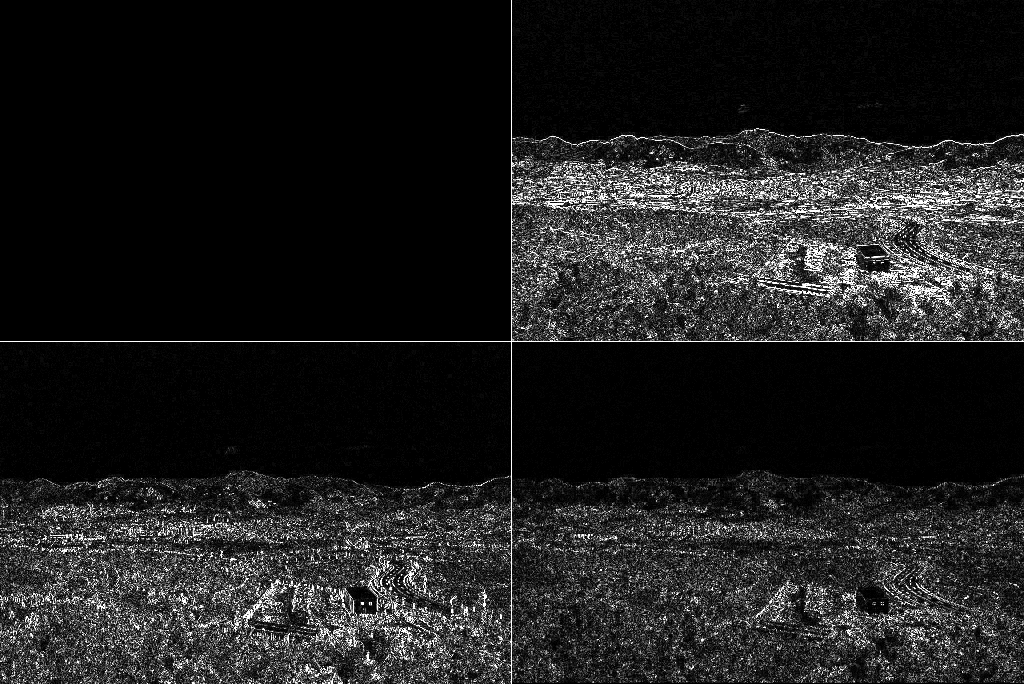
\includegraphics[scale=0.25]{n_eq_1_cut.png} 
             				\caption{消除近似分量} 
             				\label{remove_a}
             			\end{figure}
                         
             			\begin{figure}[H]
             				\centering 
             				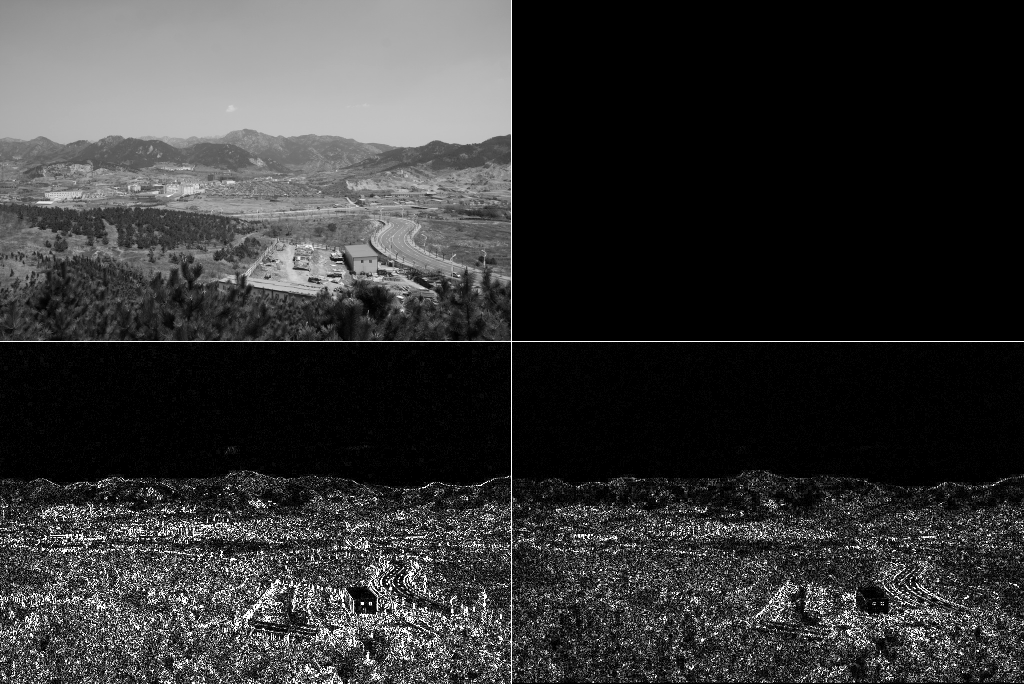
\includegraphics[scale=0.25]{n_eq_1_cut_h.png} 
             				\caption{消除水平分量} 
             				\label{remove_h}
             			\end{figure}                                          

             			\begin{figure}[H]
             				\centering 
             				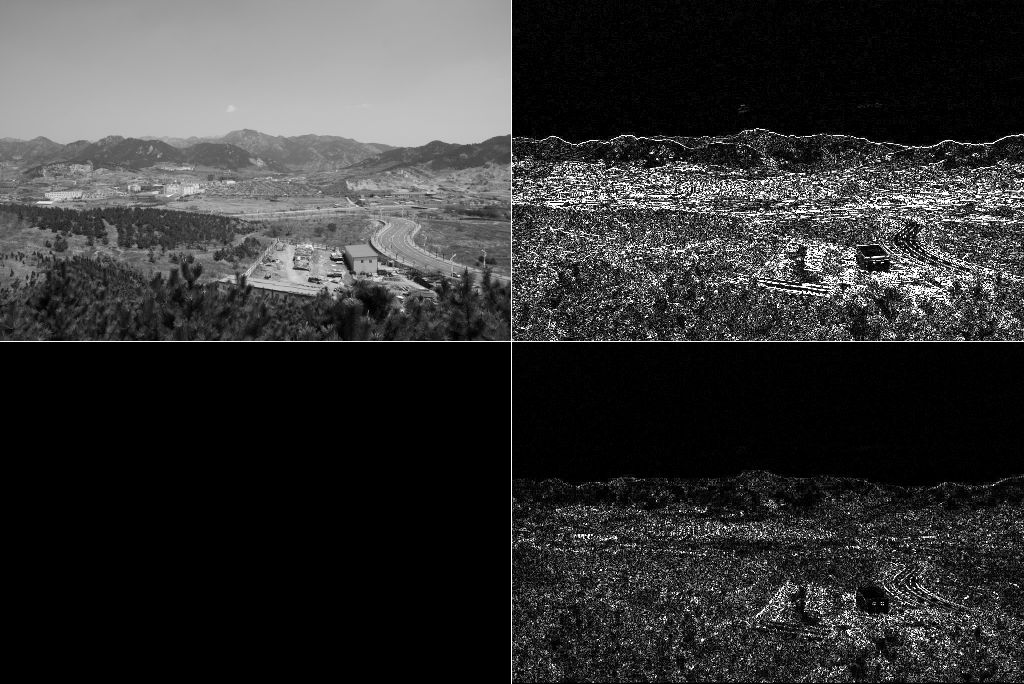
\includegraphics[scale=0.25]{n_eq_1_cut_v.png} 
             				\caption{消除垂直分量} 
             				\label{remove_v}
             			\end{figure}
                         
             			\begin{figure}[H]
             				\centering 
             				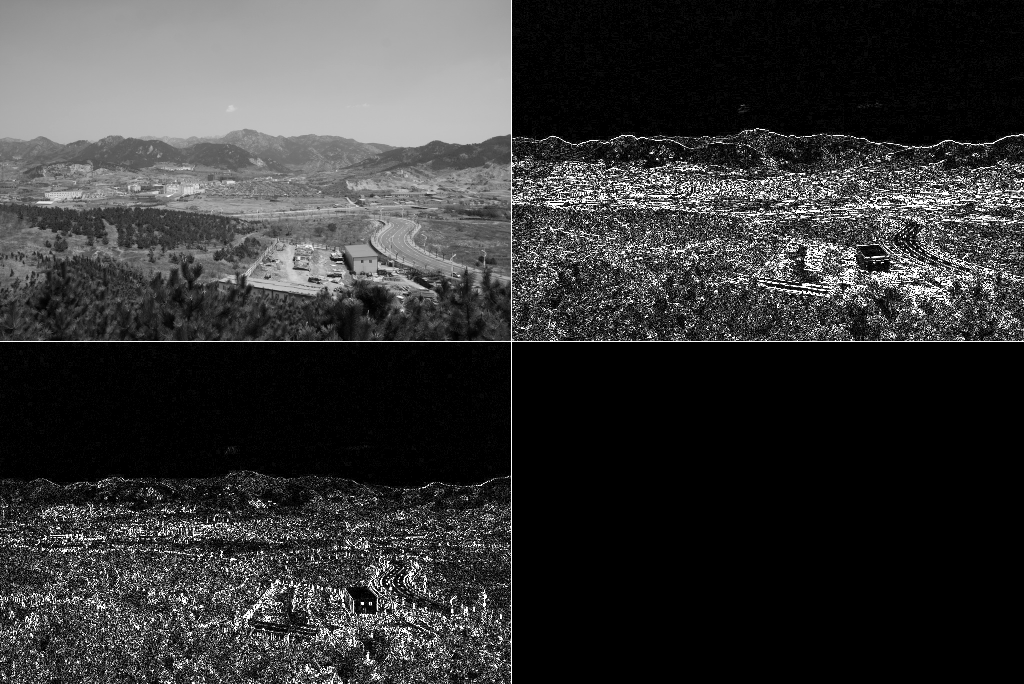
\includegraphics[scale=0.25]{n_eq_1_cut_d.png} 
             				\caption{消除对角分量} 
             				\label{remove_d}
             			\end{figure}                                             
                
                \indent 本次实验中指定消除最低尺度近似分量。 

            \subsubsection{$waveback$函数}
            
                \indent 该函数用于计算二维小波变换的反变换。输入小波系数和记录矩阵以及采用的小波类型,输出反变换结果。
                
                \indent 这里采用消除分量后的小波系数,原记录矩阵以及哈尔小波。
            
        \subsection{代码实现}
           
             \begin{lstlisting}[language=Matlab,caption={$wavetest$代码},label={broadcast.cpp}]
n = 4; % 指定阶数
n_str = num2str(n); % 将n转为字符串,用于保存图像
wave = 'haar'; % 指定变换用的小波类型

f=rgb2gray(imread('laoshan.jpg')); % 读取图像
figure,imshow(f); % 显示原图
imwrite(f, strcat('../report/', strcat(strcat('n_eq_', n_str), '_orig.png')))% 保存原图
[c,s]=wavefast(f, n, wave); % 进行二维哈尔小波变换
figure; w = wave2gray(c, s, -6); % 显示小波系数
imwrite(w, strcat('../report/', strcat(strcat('n_eq_', n_str), '_FWT.png')))% 保存变换结果
[nc,y]=wavecut('a', c, s); % 消除指定分量
figure, w = wave2gray(nc, s, -6); % 显示消除分量后的小波系数
imwrite(w, strcat('../report/', strcat(strcat('n_eq_', n_str), '_cut.png')))% 保存消除分量后的结果
edge=abs(waveback(nc, s, wave)); % 进行反变换
figure,imshow(mat2gray(edge)); % 显示反变换后的结果
imwrite(mat2gray(edge), strcat('../report/', strcat(strcat('n_eq_', n_str), '_edge.png')))% 保存变换结果


              \end{lstlisting}
    

        \subsection{结果展示}
        

                        
                        \begin{figure}[H]
                            \centering
                            \subfigure[原图的灰度图]{
                                \begin{minipage}{0.45\linewidth}
                                    \centering
                                    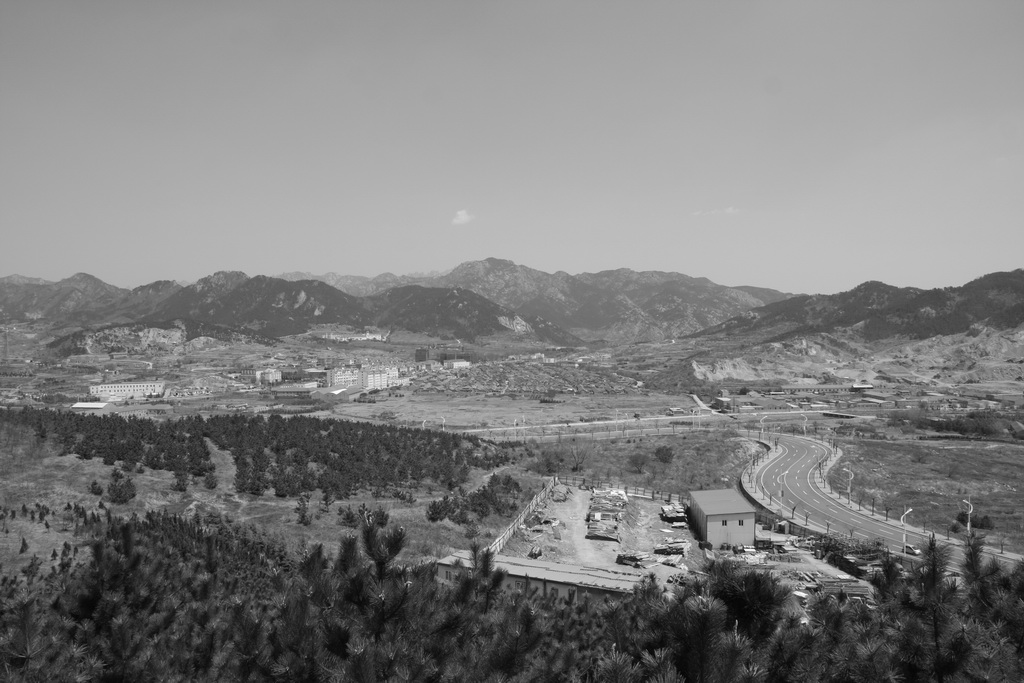
\includegraphics[scale=0.2]{n_eq_4_orig.png}
                                    %\caption{原图3}
                                \end{minipage}
                            }
                            \subfigure[小波变换结果]{
                                \begin{minipage}{0.45\linewidth}
                                    \centering
                                    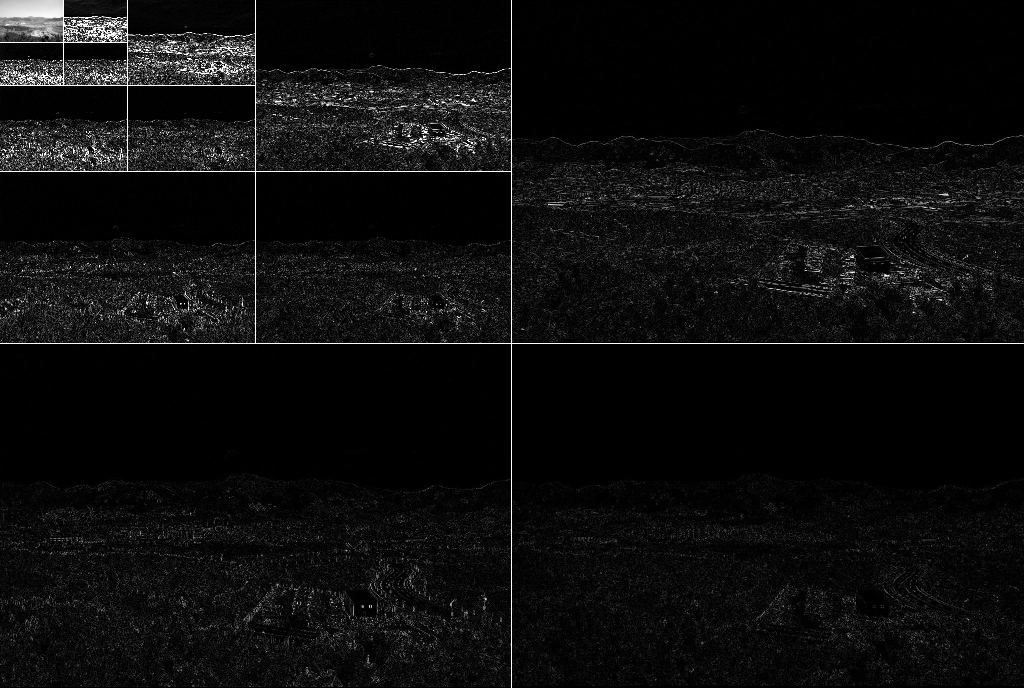
\includegraphics[scale=0.2]{n_eq_4_FWT.png}
                                    %\caption{结果3}
                                    \label{n_eq_4_FWT}
                                \end{minipage}
                            }
                            \subfigure[消除近似分量后的变换结果]{
                                \begin{minipage}{0.45\linewidth}
                                    \centering
                                    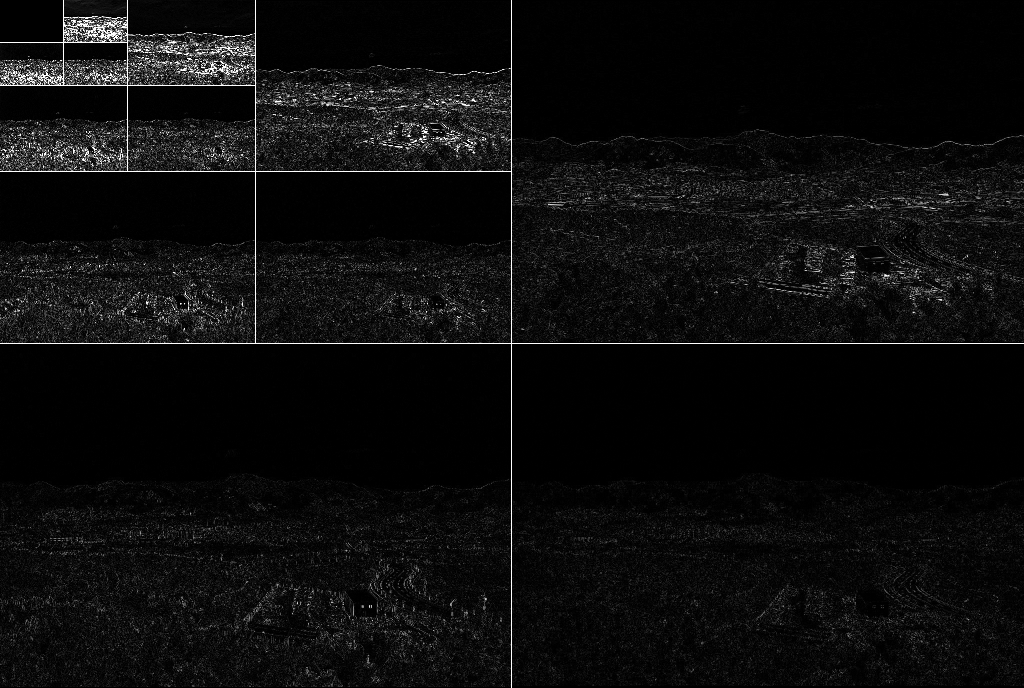
\includegraphics[scale=0.2]{n_eq_4_cut.png}
                                    %\caption{结果3}
                                    \label{n_eq_4_cut}
                                \end{minipage}
                            }  
                            \subfigure[反变换后的结果:边缘增强]{
                                \begin{minipage}{0.45\linewidth}
                                    \centering
                                    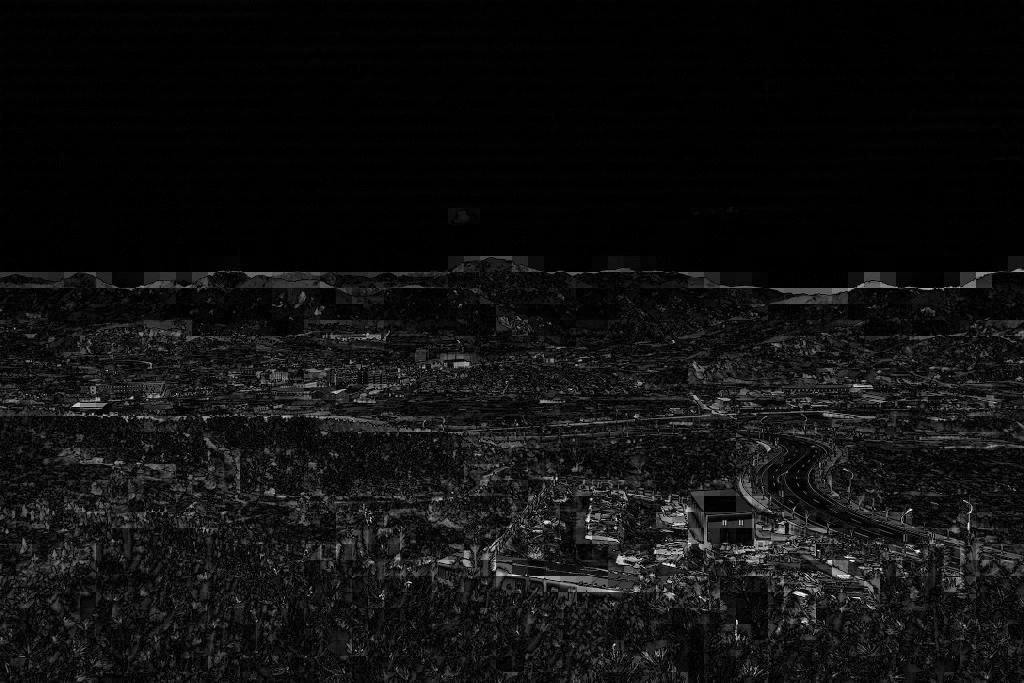
\includegraphics[scale=0.2]{n_eq_4_edge.png}
                                    %\caption{结果3}
                                    \label{n_eq_4_edge}
                                \end{minipage}
                            }                                                      
                            
                            \caption{$n$等于$4$时的实验结果}
                            \label{n_eq_4}
                        \end{figure}
                        
                        
                        \begin{figure}[H]
                            \centering
                            \subfigure[原图的灰度图]{
                                \begin{minipage}{0.45\linewidth}
                                    \centering
                                    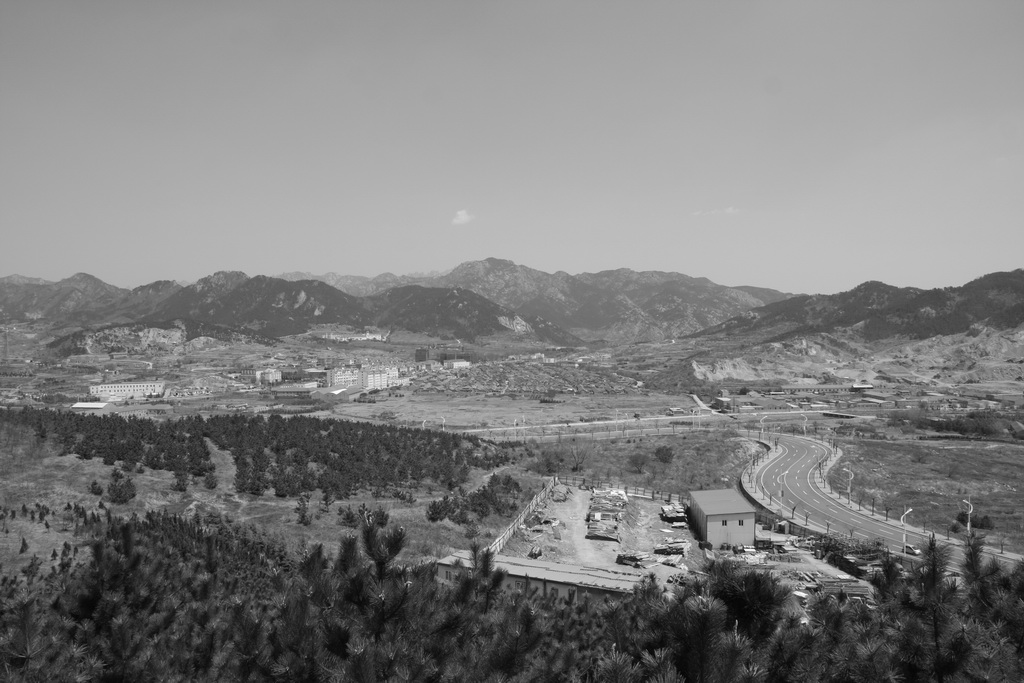
\includegraphics[scale=0.2]{n_eq_1_orig.png}
                                    %\caption{原图3}
                                \end{minipage}
                            }
                            \subfigure[小波变换结果]{
                                \begin{minipage}{0.45\linewidth}
                                    \centering
                                    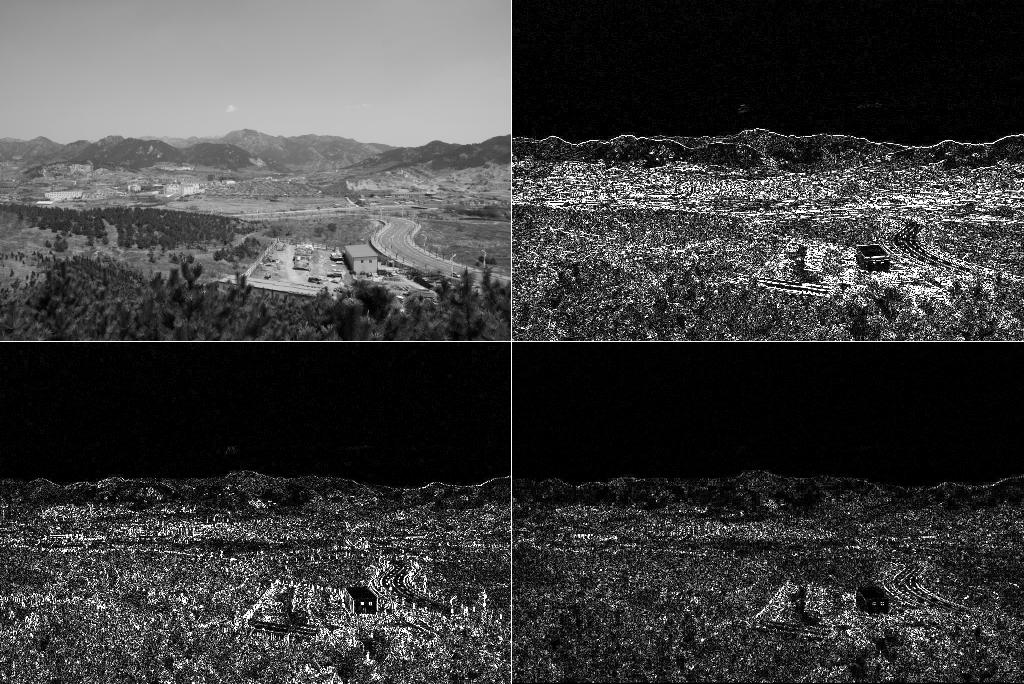
\includegraphics[scale=0.2]{n_eq_1_FWT.png}
                                    %\caption{结果3}
                                    \label{n_eq_1_FWT}
                                \end{minipage}
                            }
                            \subfigure[消除近似分量后的变换结果]{
                                \begin{minipage}{0.45\linewidth}
                                    \centering
                                    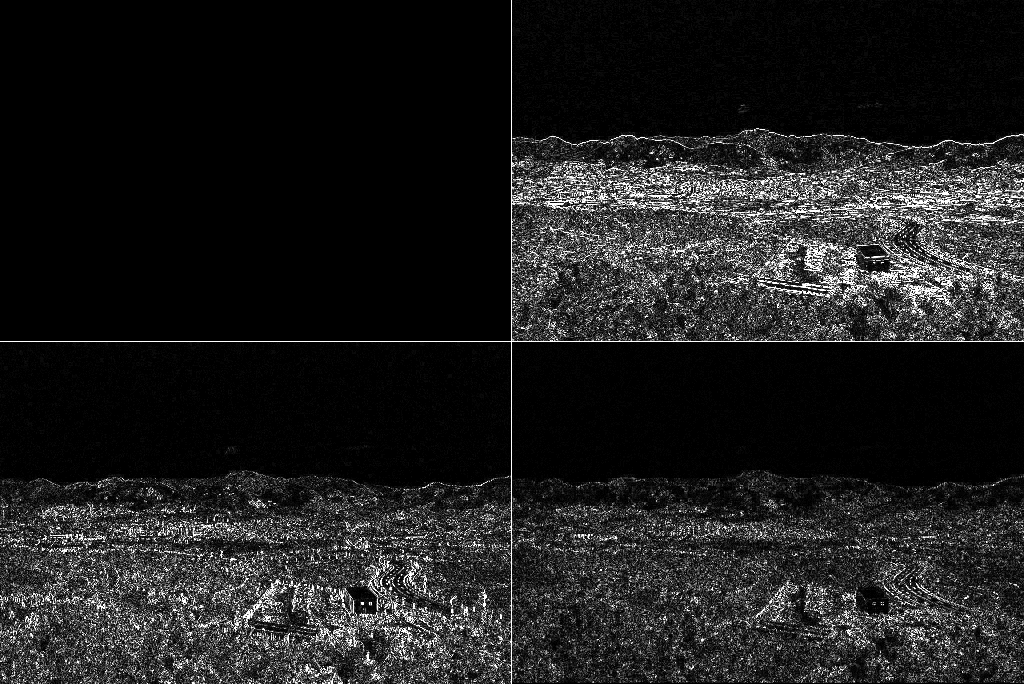
\includegraphics[scale=0.2]{n_eq_1_cut.png}
                                    %\caption{结果3}
                                    \label{n_eq_1_cut}
                                \end{minipage}
                            }  
                            \subfigure[反变换后的结果:边缘增强]{
                                \begin{minipage}{0.45\linewidth}
                                    \centering
                                    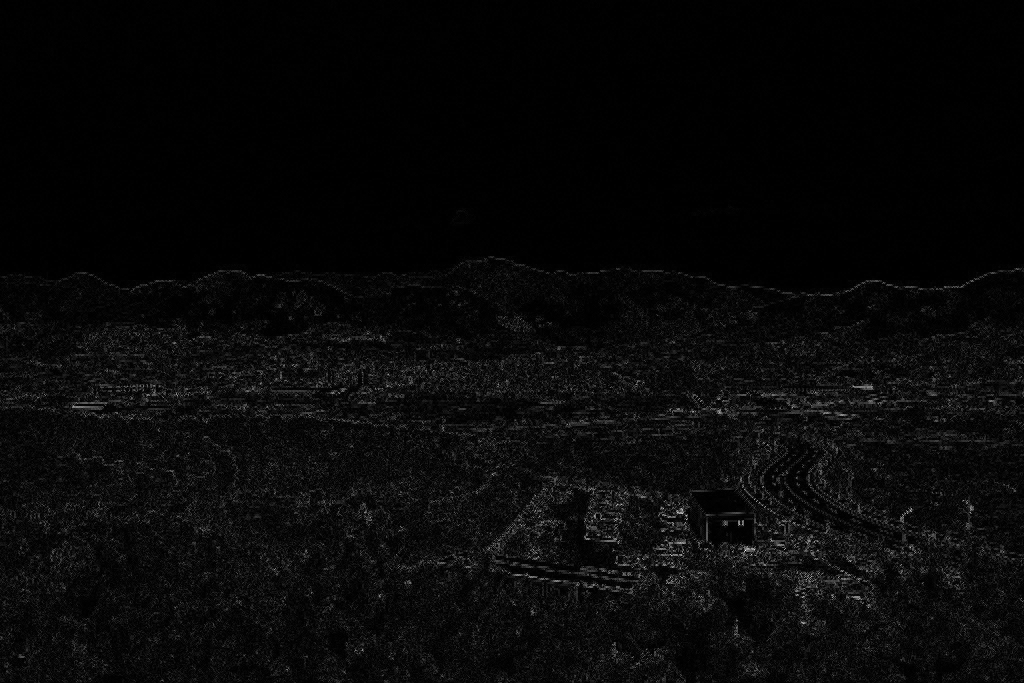
\includegraphics[scale=0.2]{n_eq_1_edge.png}
                                    %\caption{结果3}
                                    \label{n_eq_1_edge}
                                \end{minipage}
                            }                                                      
                            
                            \caption{$n$等于$1$时的实验结果}
                            \label{n_eq_1}
                        \end{figure} 
                                               
                        \begin{figure}[H]
                            \centering
                            \subfigure[原图的灰度图]{
                                \begin{minipage}{0.45\linewidth}
                                    \centering
                                    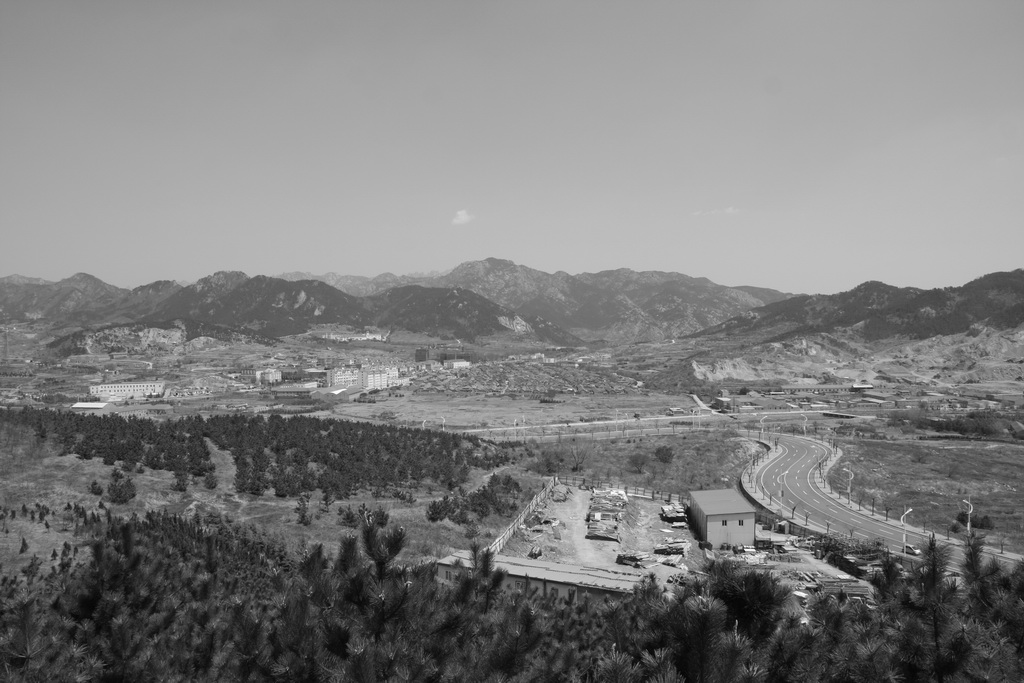
\includegraphics[scale=0.2]{n_eq_2_orig.png}
                                    %\caption{原图3}
                                \end{minipage}
                            }
                            \subfigure[小波变换结果]{
                                \begin{minipage}{0.45\linewidth}
                                    \centering
                                    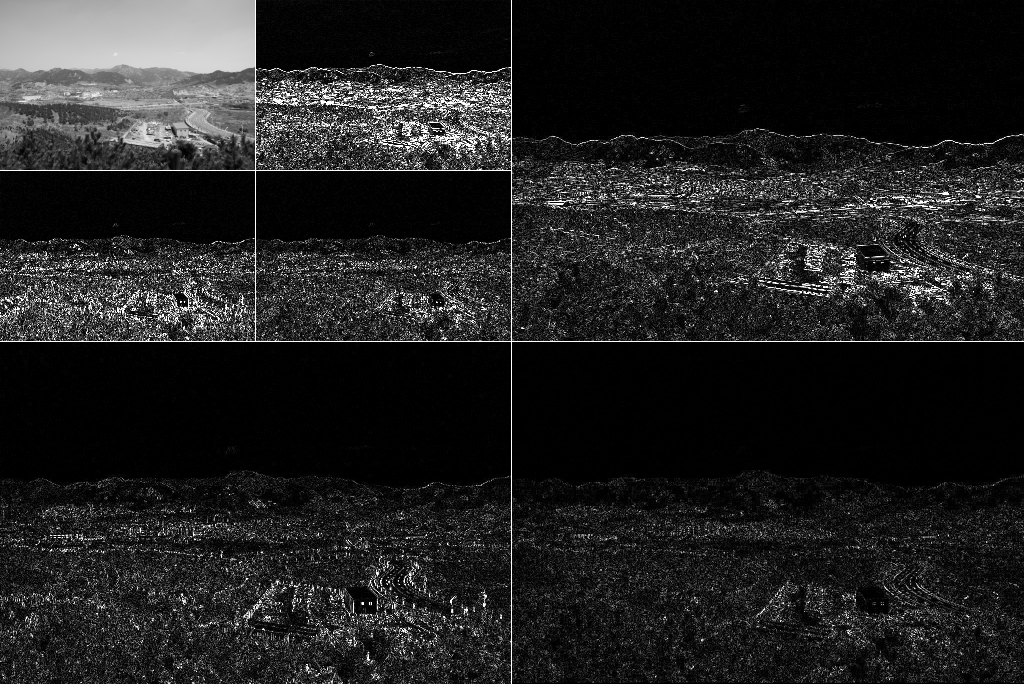
\includegraphics[scale=0.2]{n_eq_2_FWT.png}
                                    %\caption{结果3}
                                    \label{n_eq_2_FWT}
                                \end{minipage}
                            }
                            \subfigure[消除近似分量后的变换结果]{
                                \begin{minipage}{0.45\linewidth}
                                    \centering
                                    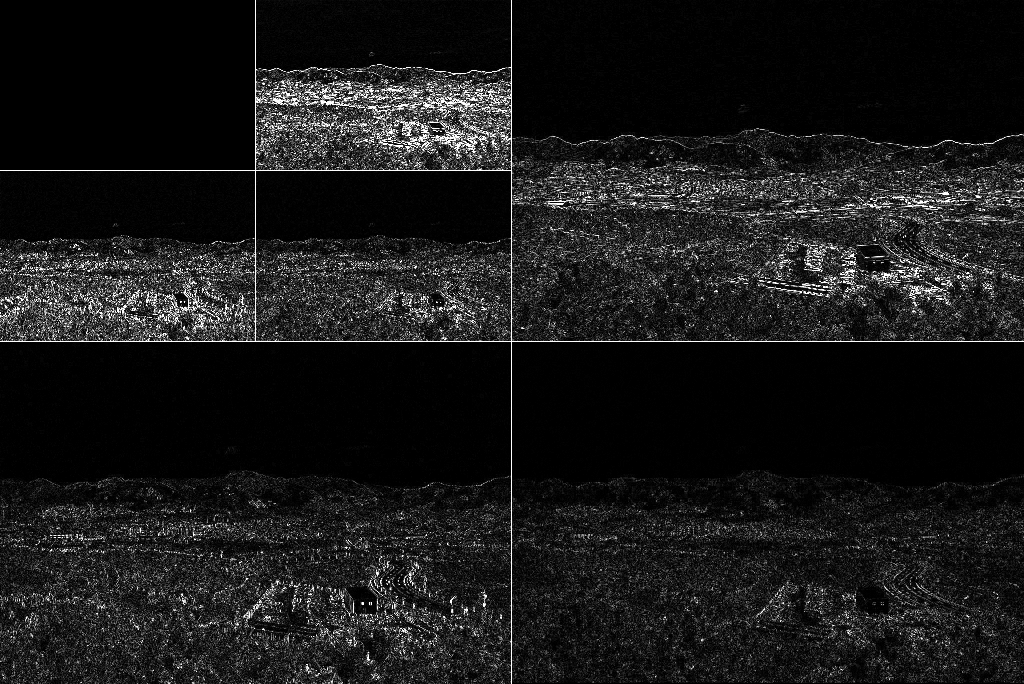
\includegraphics[scale=0.2]{n_eq_2_cut.png}
                                    %\caption{结果3}
                                    \label{n_eq_2_cut}
                                \end{minipage}
                            }  
                            \subfigure[反变换后的结果:边缘增强]{
                                \begin{minipage}{0.45\linewidth}
                                    \centering
                                    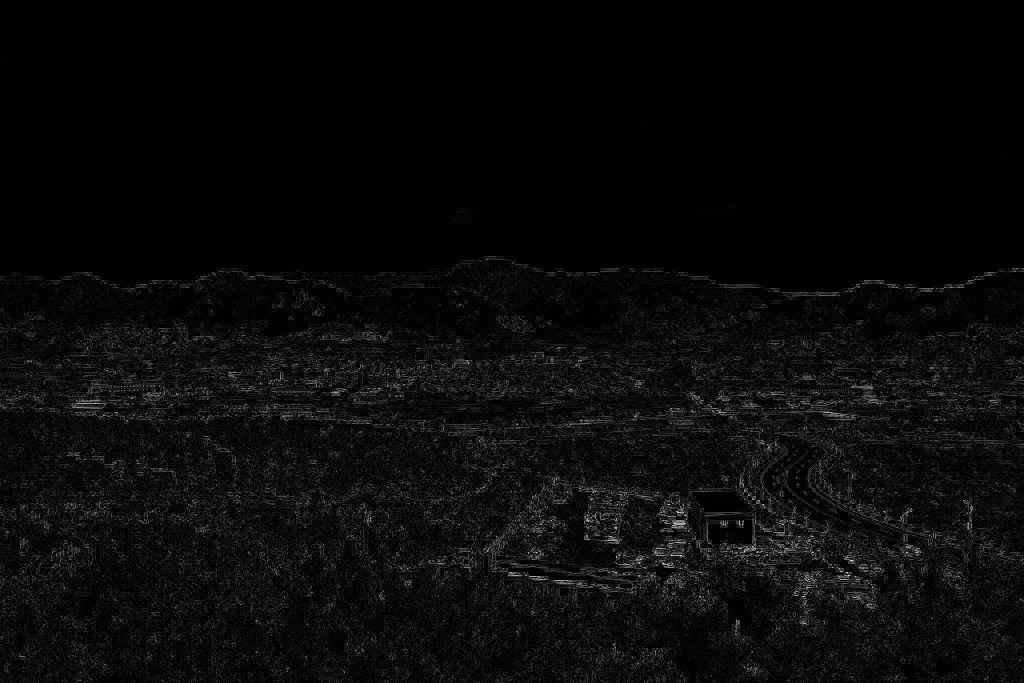
\includegraphics[scale=0.2]{n_eq_2_edge.png}
                                    %\caption{结果3}
                                    \label{n_eq_2_edge}
                                \end{minipage}
                            }                                                      
                            
                            \caption{$n$等于$2$时的实验结果}
                            \label{n_eq_2}
                        \end{figure}

                        \begin{figure}[H]
                            \centering
                            \subfigure[原图的灰度图]{
                                \begin{minipage}{0.45\linewidth}
                                    \centering
                                    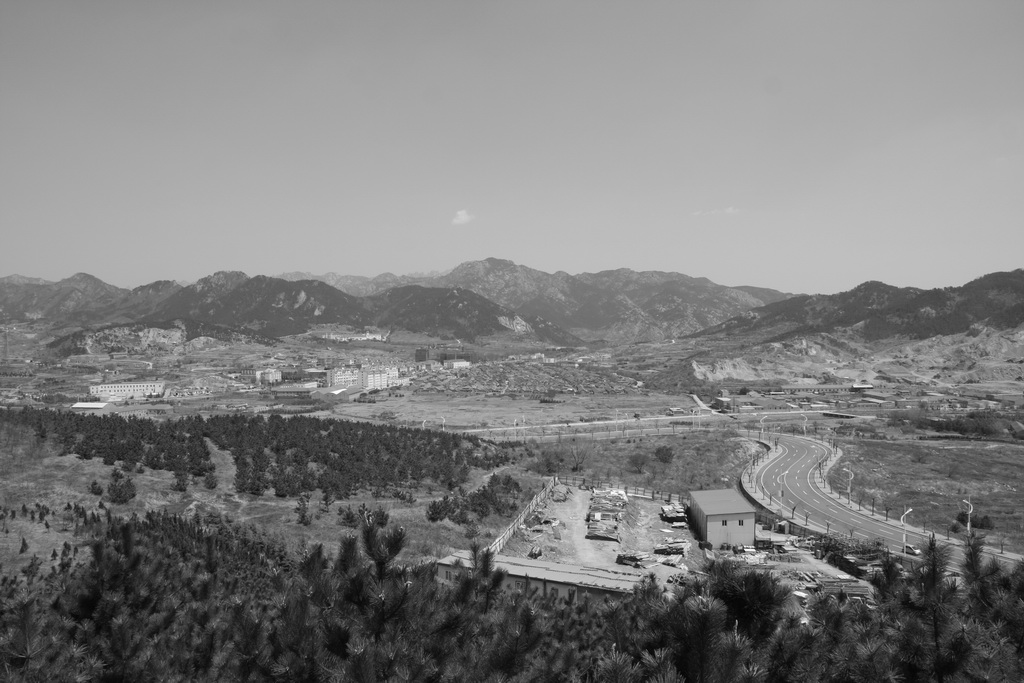
\includegraphics[scale=0.2]{n_eq_8_orig.png}
                                    %\caption{原图3}
                                \end{minipage}
                            }
                            \subfigure[小波变换结果]{
                                \begin{minipage}{0.45\linewidth}
                                    \centering
                                    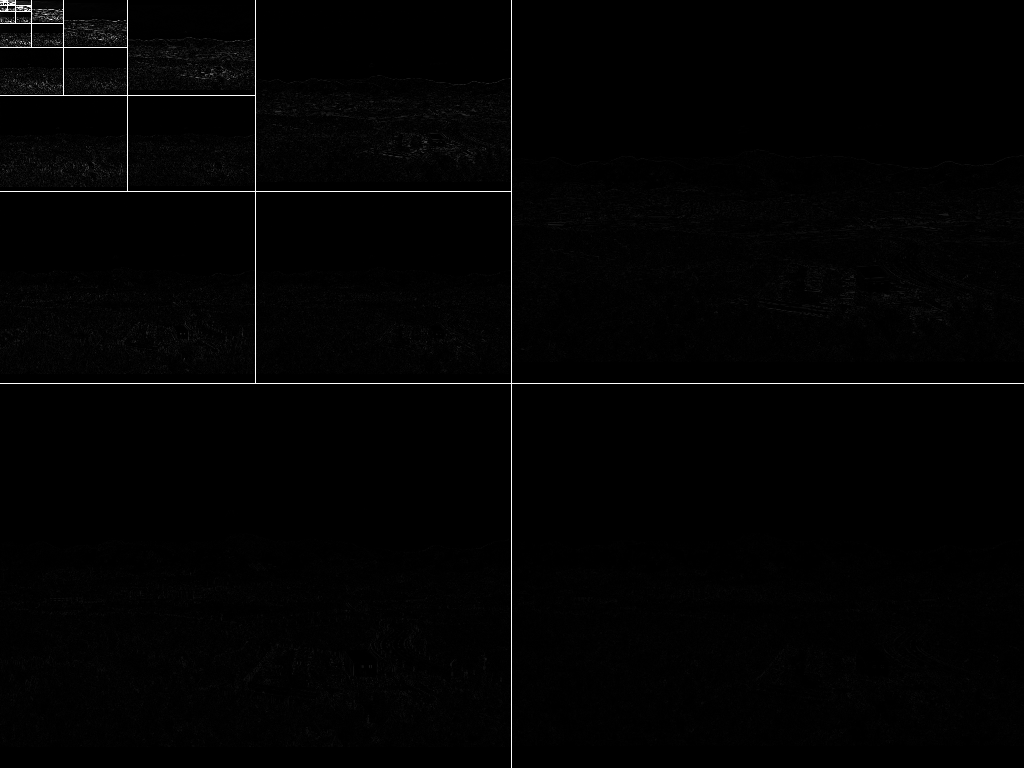
\includegraphics[scale=0.2]{n_eq_8_FWT.png}
                                    %\caption{结果3}
                                    \label{n_eq_8_FWT}
                                \end{minipage}
                            }
                            \subfigure[消除近似分量后的变换结果]{
                                \begin{minipage}{0.45\linewidth}
                                    \centering
                                    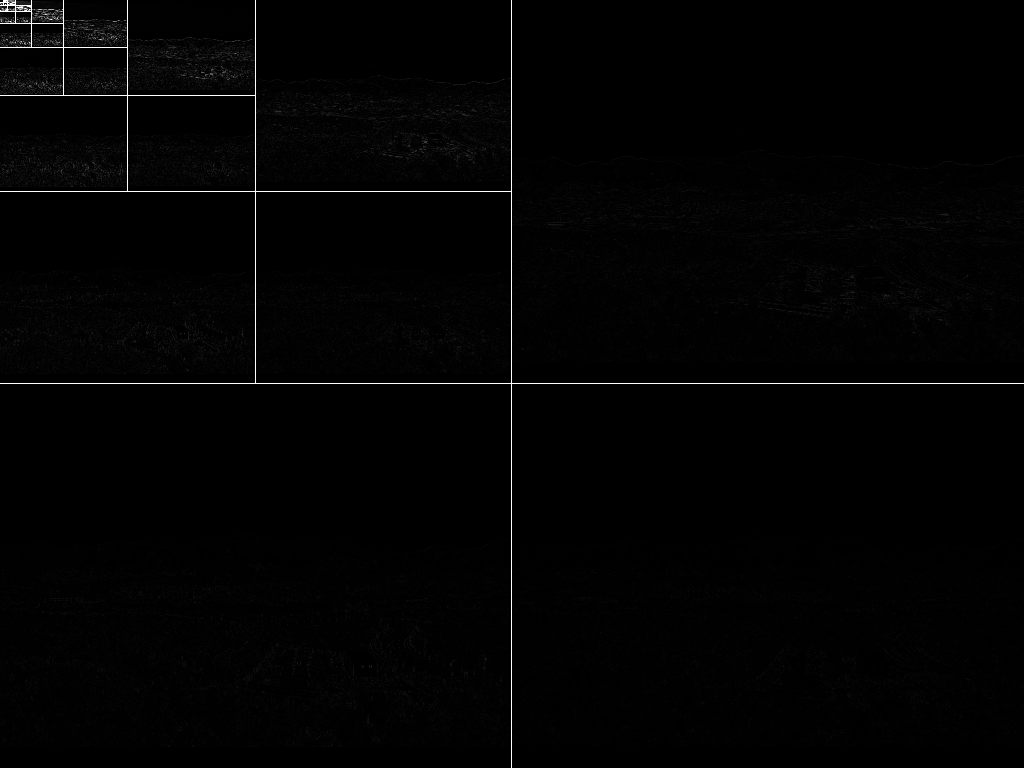
\includegraphics[scale=0.2]{n_eq_8_cut.png}
                                    %\caption{结果3}
                                    \label{n_eq_8_cut}
                                \end{minipage}
                            }  
                            \subfigure[反变换后的结果:边缘增强]{
                                \begin{minipage}{0.45\linewidth}
                                    \centering
                                    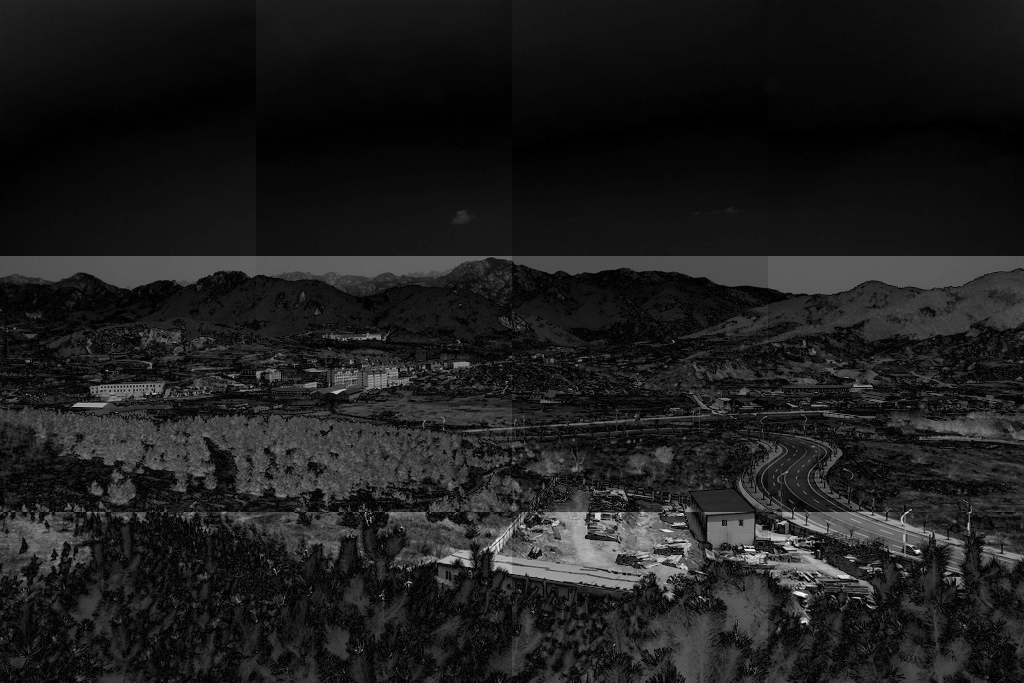
\includegraphics[scale=0.2]{n_eq_8_edge.png}
                                    %\caption{结果3}
                                    \label{n_eq_8_edge}
                                \end{minipage}
                            }                                                      
                            
                            \caption{$n$等于$8$时的实验结果}
                            \label{n_eq_8}
                        \end{figure}

                        \begin{figure}[H]
                            \centering
                            \subfigure[原图的灰度图]{
                                \begin{minipage}{0.45\linewidth}
                                    \centering
                                    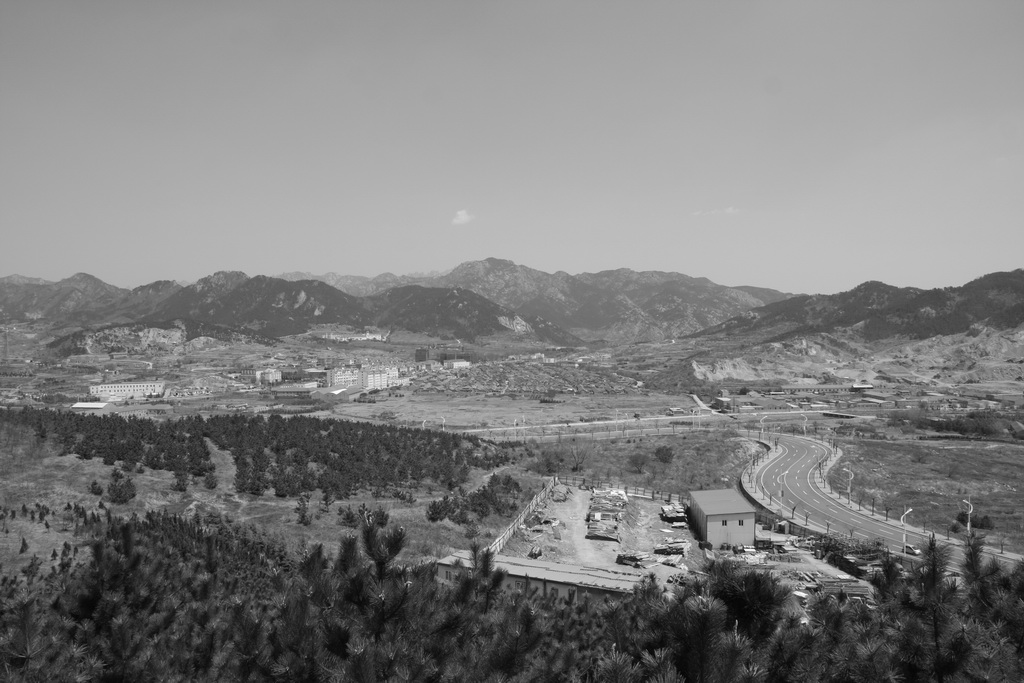
\includegraphics[scale=0.2]{n_eq_10_orig.png}
                                    %\caption{原图3}
                                \end{minipage}
                            }
                            \subfigure[小波变换结果]{
                                \begin{minipage}{0.45\linewidth}
                                    \centering
                                    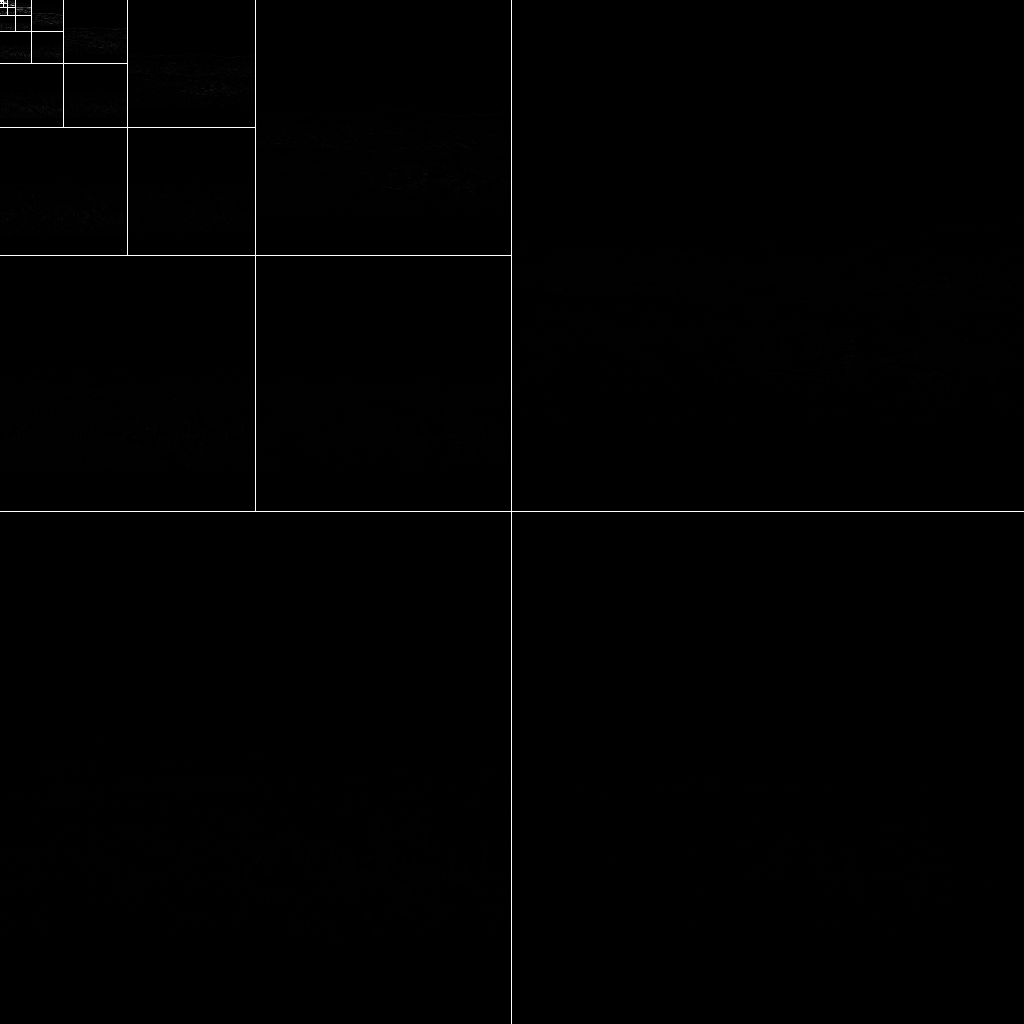
\includegraphics[scale=0.2]{n_eq_10_FWT.png}
                                    %\caption{结果3}
                                    \label{n_eq_10_FWT}
                                \end{minipage}
                            }
                            \subfigure[消除近似分量后的变换结果]{
                                \begin{minipage}{0.45\linewidth}
                                    \centering
                                    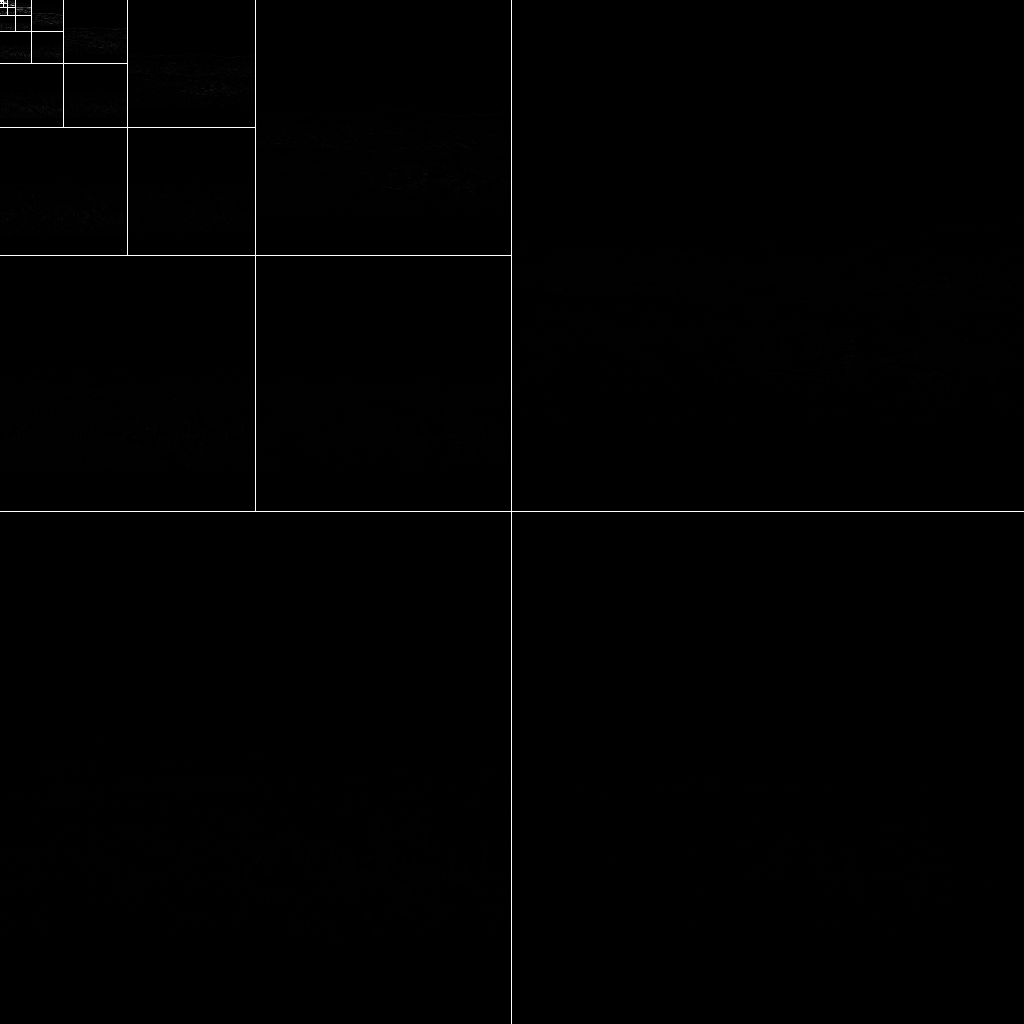
\includegraphics[scale=0.2]{n_eq_10_cut.png}
                                    %\caption{结果3}
                                    \label{n_eq_10_cut}
                                \end{minipage}
                            }  
                            \subfigure[反变换后的结果:边缘增强]{
                                \begin{minipage}{0.45\linewidth}
                                    \centering
                                    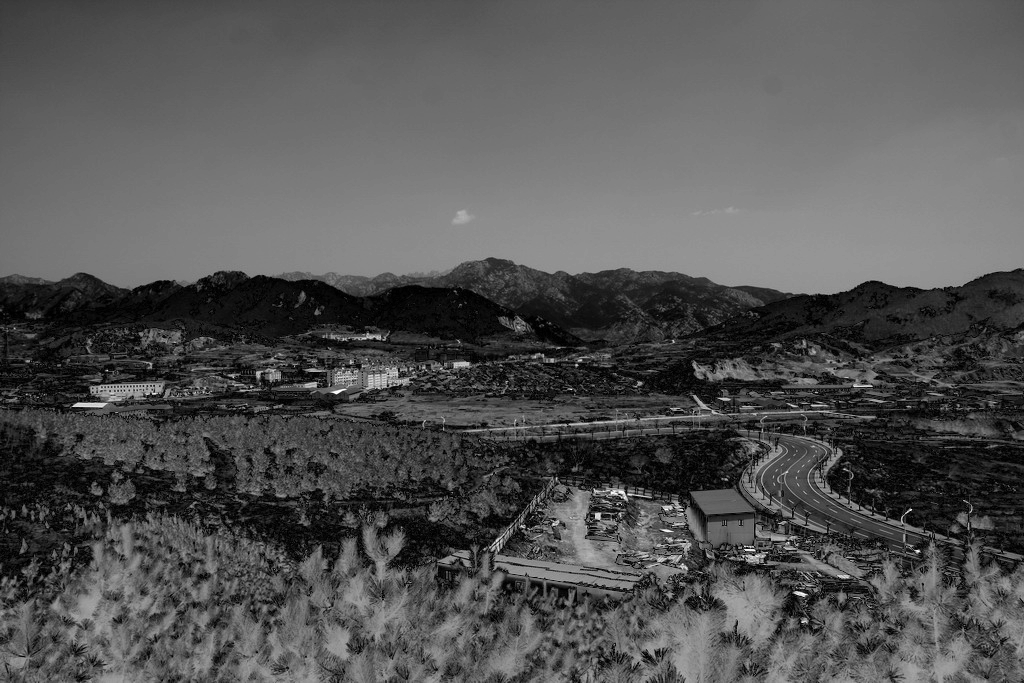
\includegraphics[scale=0.2]{n_eq_10_edge.png}
                                    %\caption{结果3}
                                    \label{n_eq_10_edge}
                                \end{minipage}
                            }                                                      
                            
                            \caption{$n$等于$10$时的实验结果}
                            \label{n_eq_10}
                        \end{figure}
                        
%                        
%        
                       
%
%                        \begin{figure}[H]
%                            \centering
%                            \subfigure[巴特沃斯带阻滤波后的图像]{
%                                \begin{minipage}{0.45\linewidth}
%                                    \centering
%                                    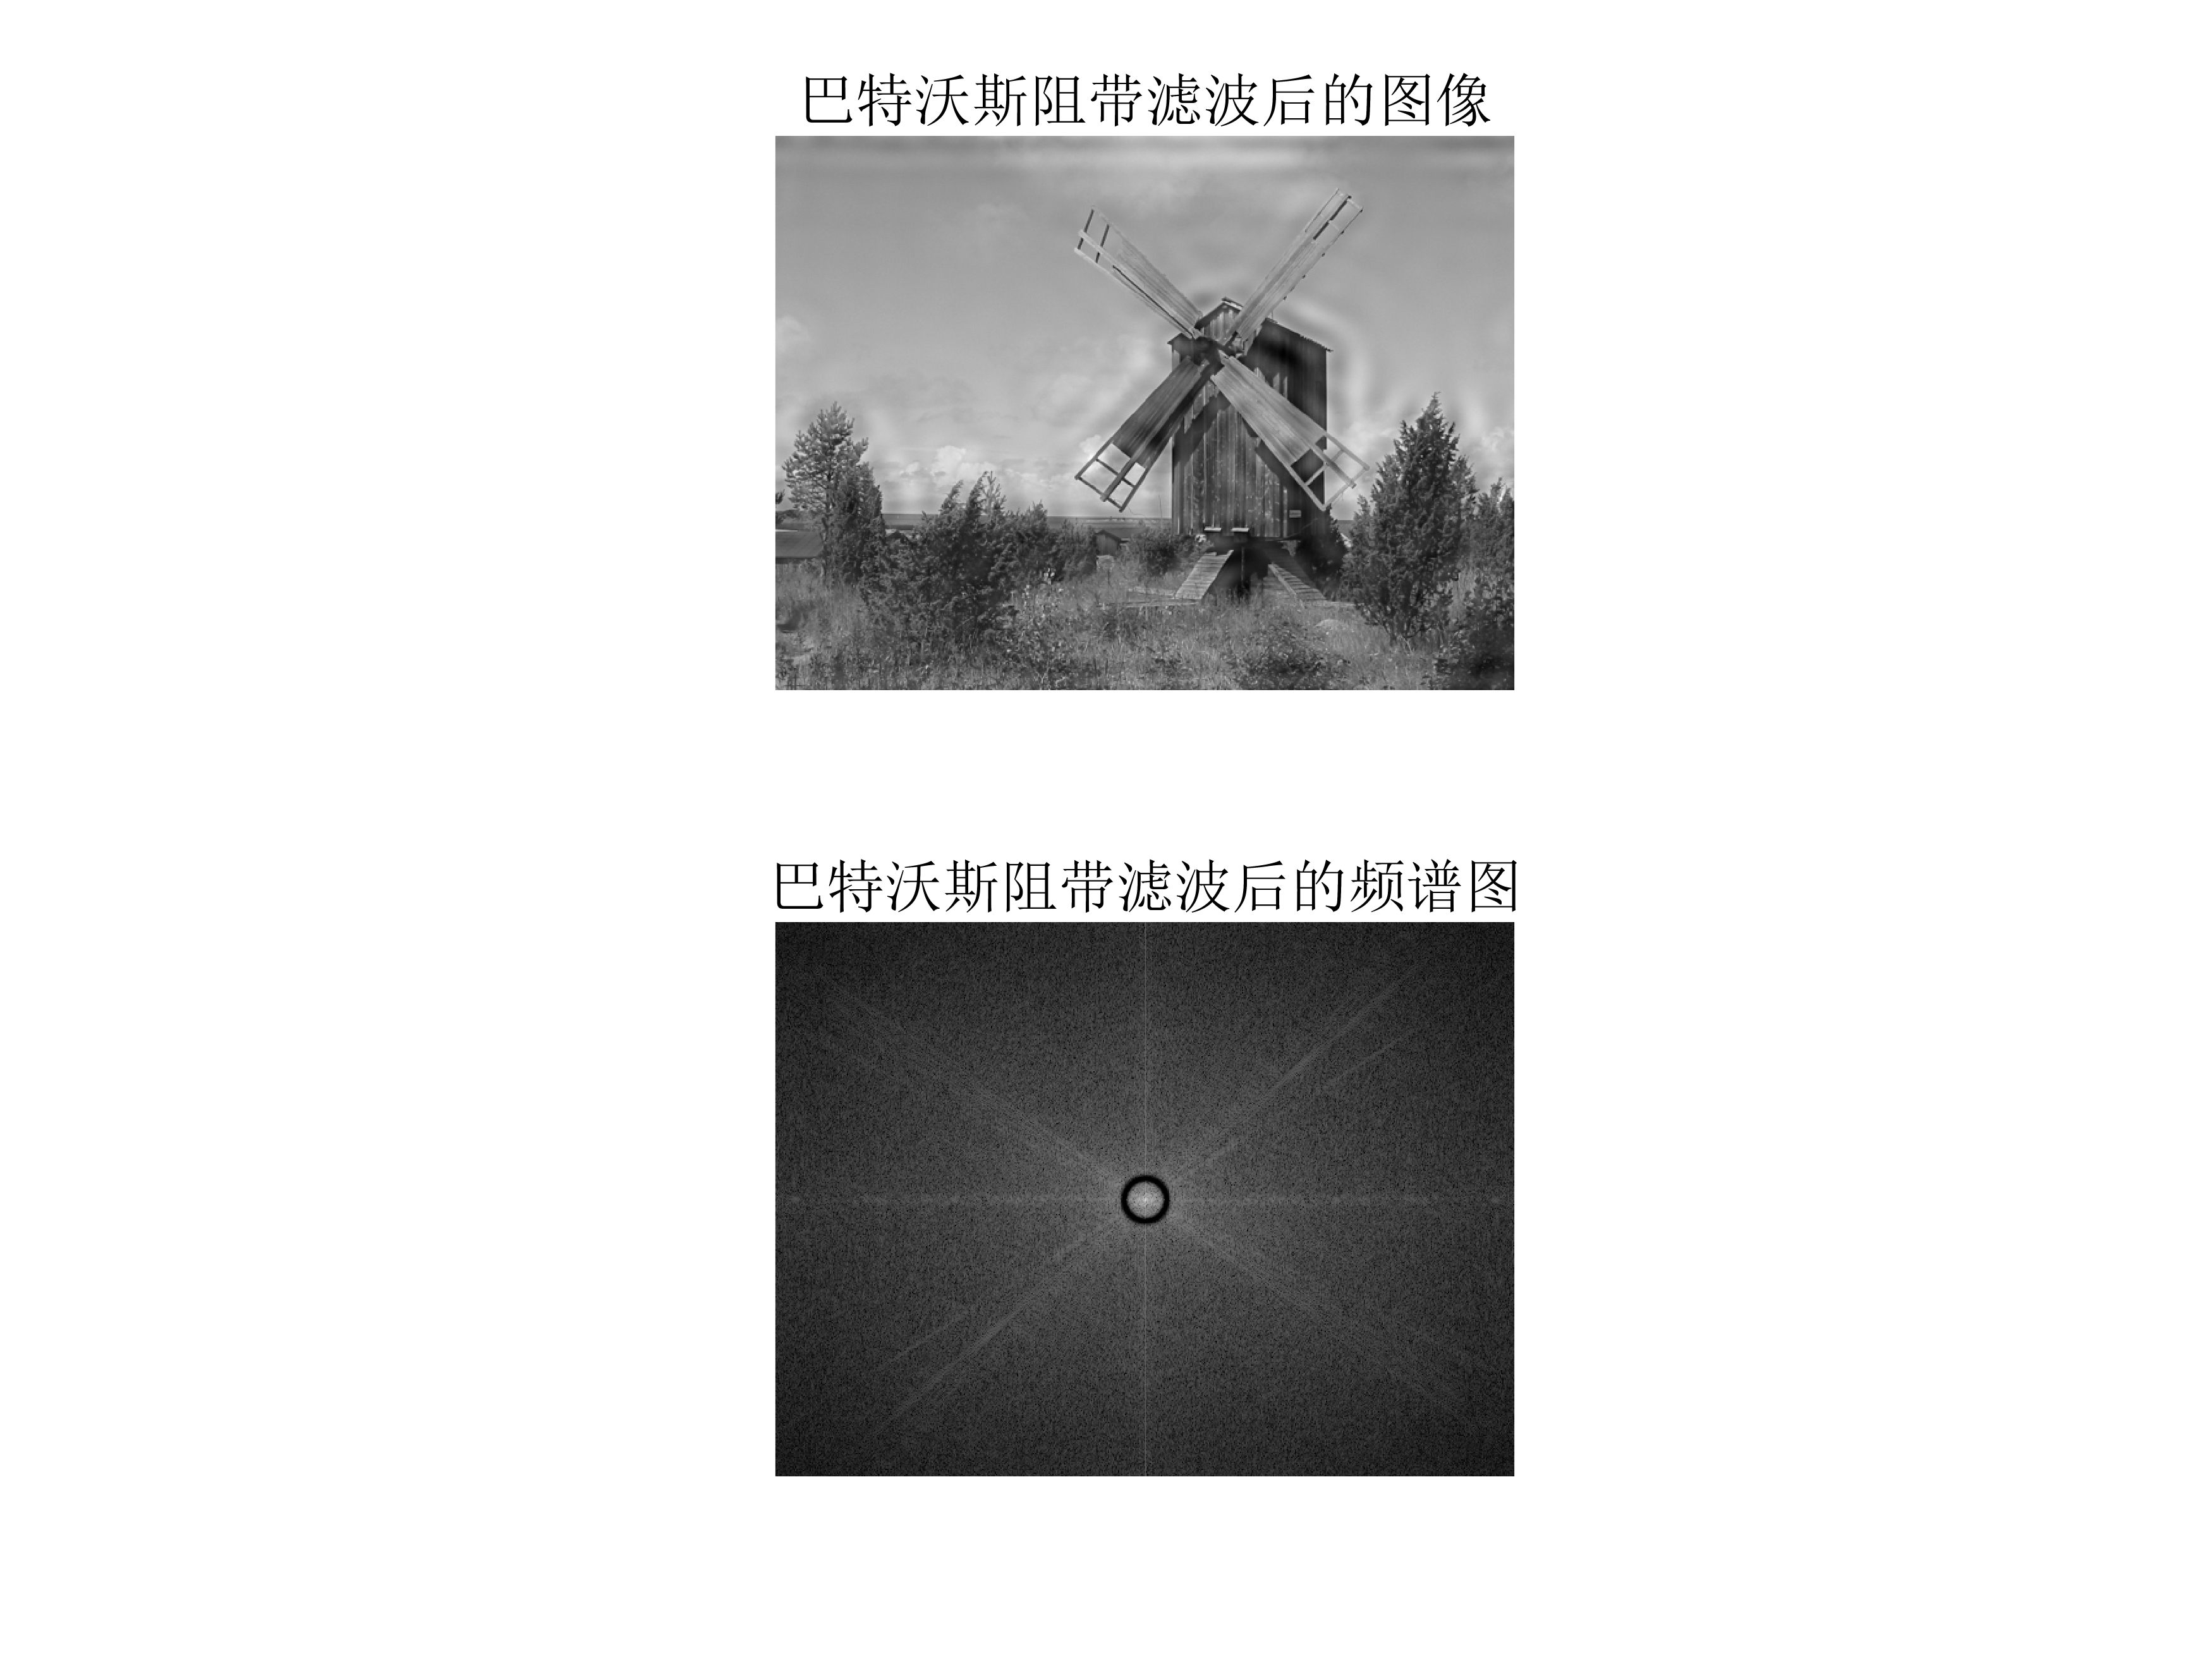
\includegraphics[scale=0.4]{./filtered_img.png}
%                                    %\caption{原图3}
%                                \end{minipage}
%                            }
%                            \subfigure[巴特沃斯带阻滤波后的频谱图]{
%                                \begin{minipage}{0.45\linewidth}
%                                    \centering
%                                    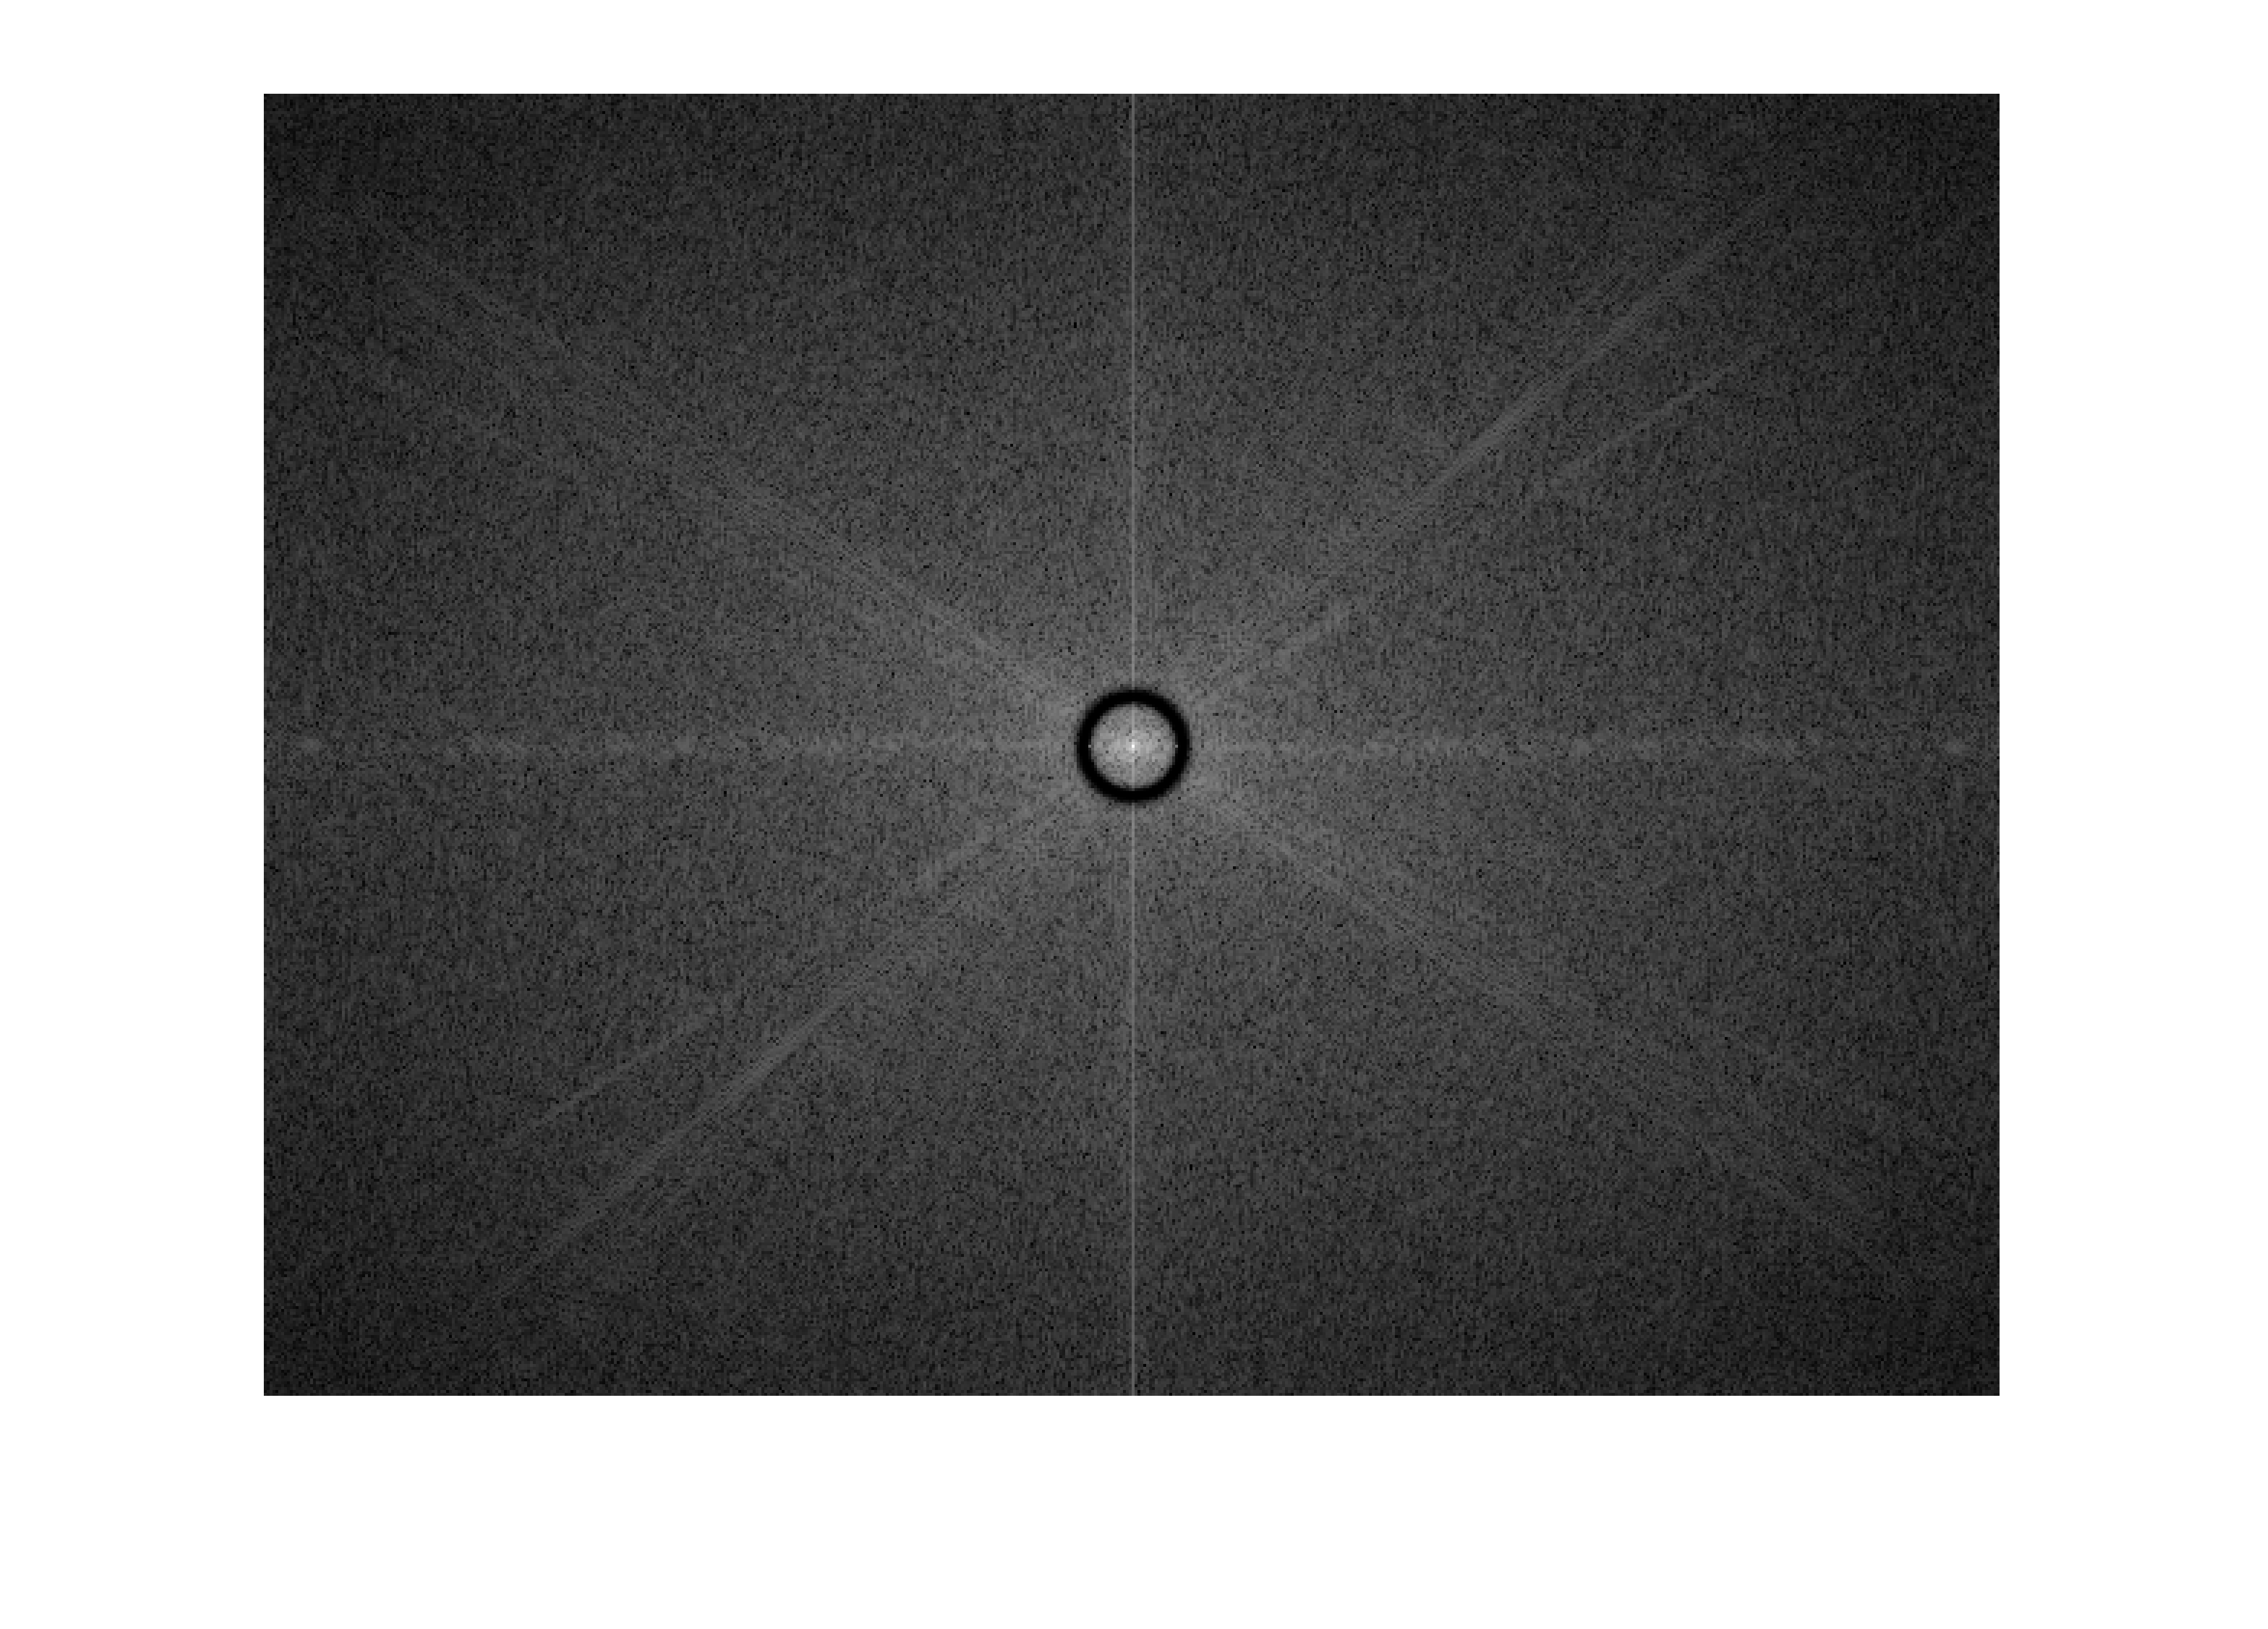
\includegraphics[scale=0.4]{./filtered_spectrum.png}
%                                    %\caption{结果3}
%                                    \label{res4-4}
%                                \end{minipage}
%                            }
%                            
%                            \caption{测试结果}
%                            \label{butterworth}
%                        \end{figure}                        
%                      
%                        \begin{figure}[H]
%                            \centering
%                            \subfigure[高斯带阻滤波后的图像]{
%                                \begin{minipage}{0.45\linewidth}
%                                    \centering
%                                    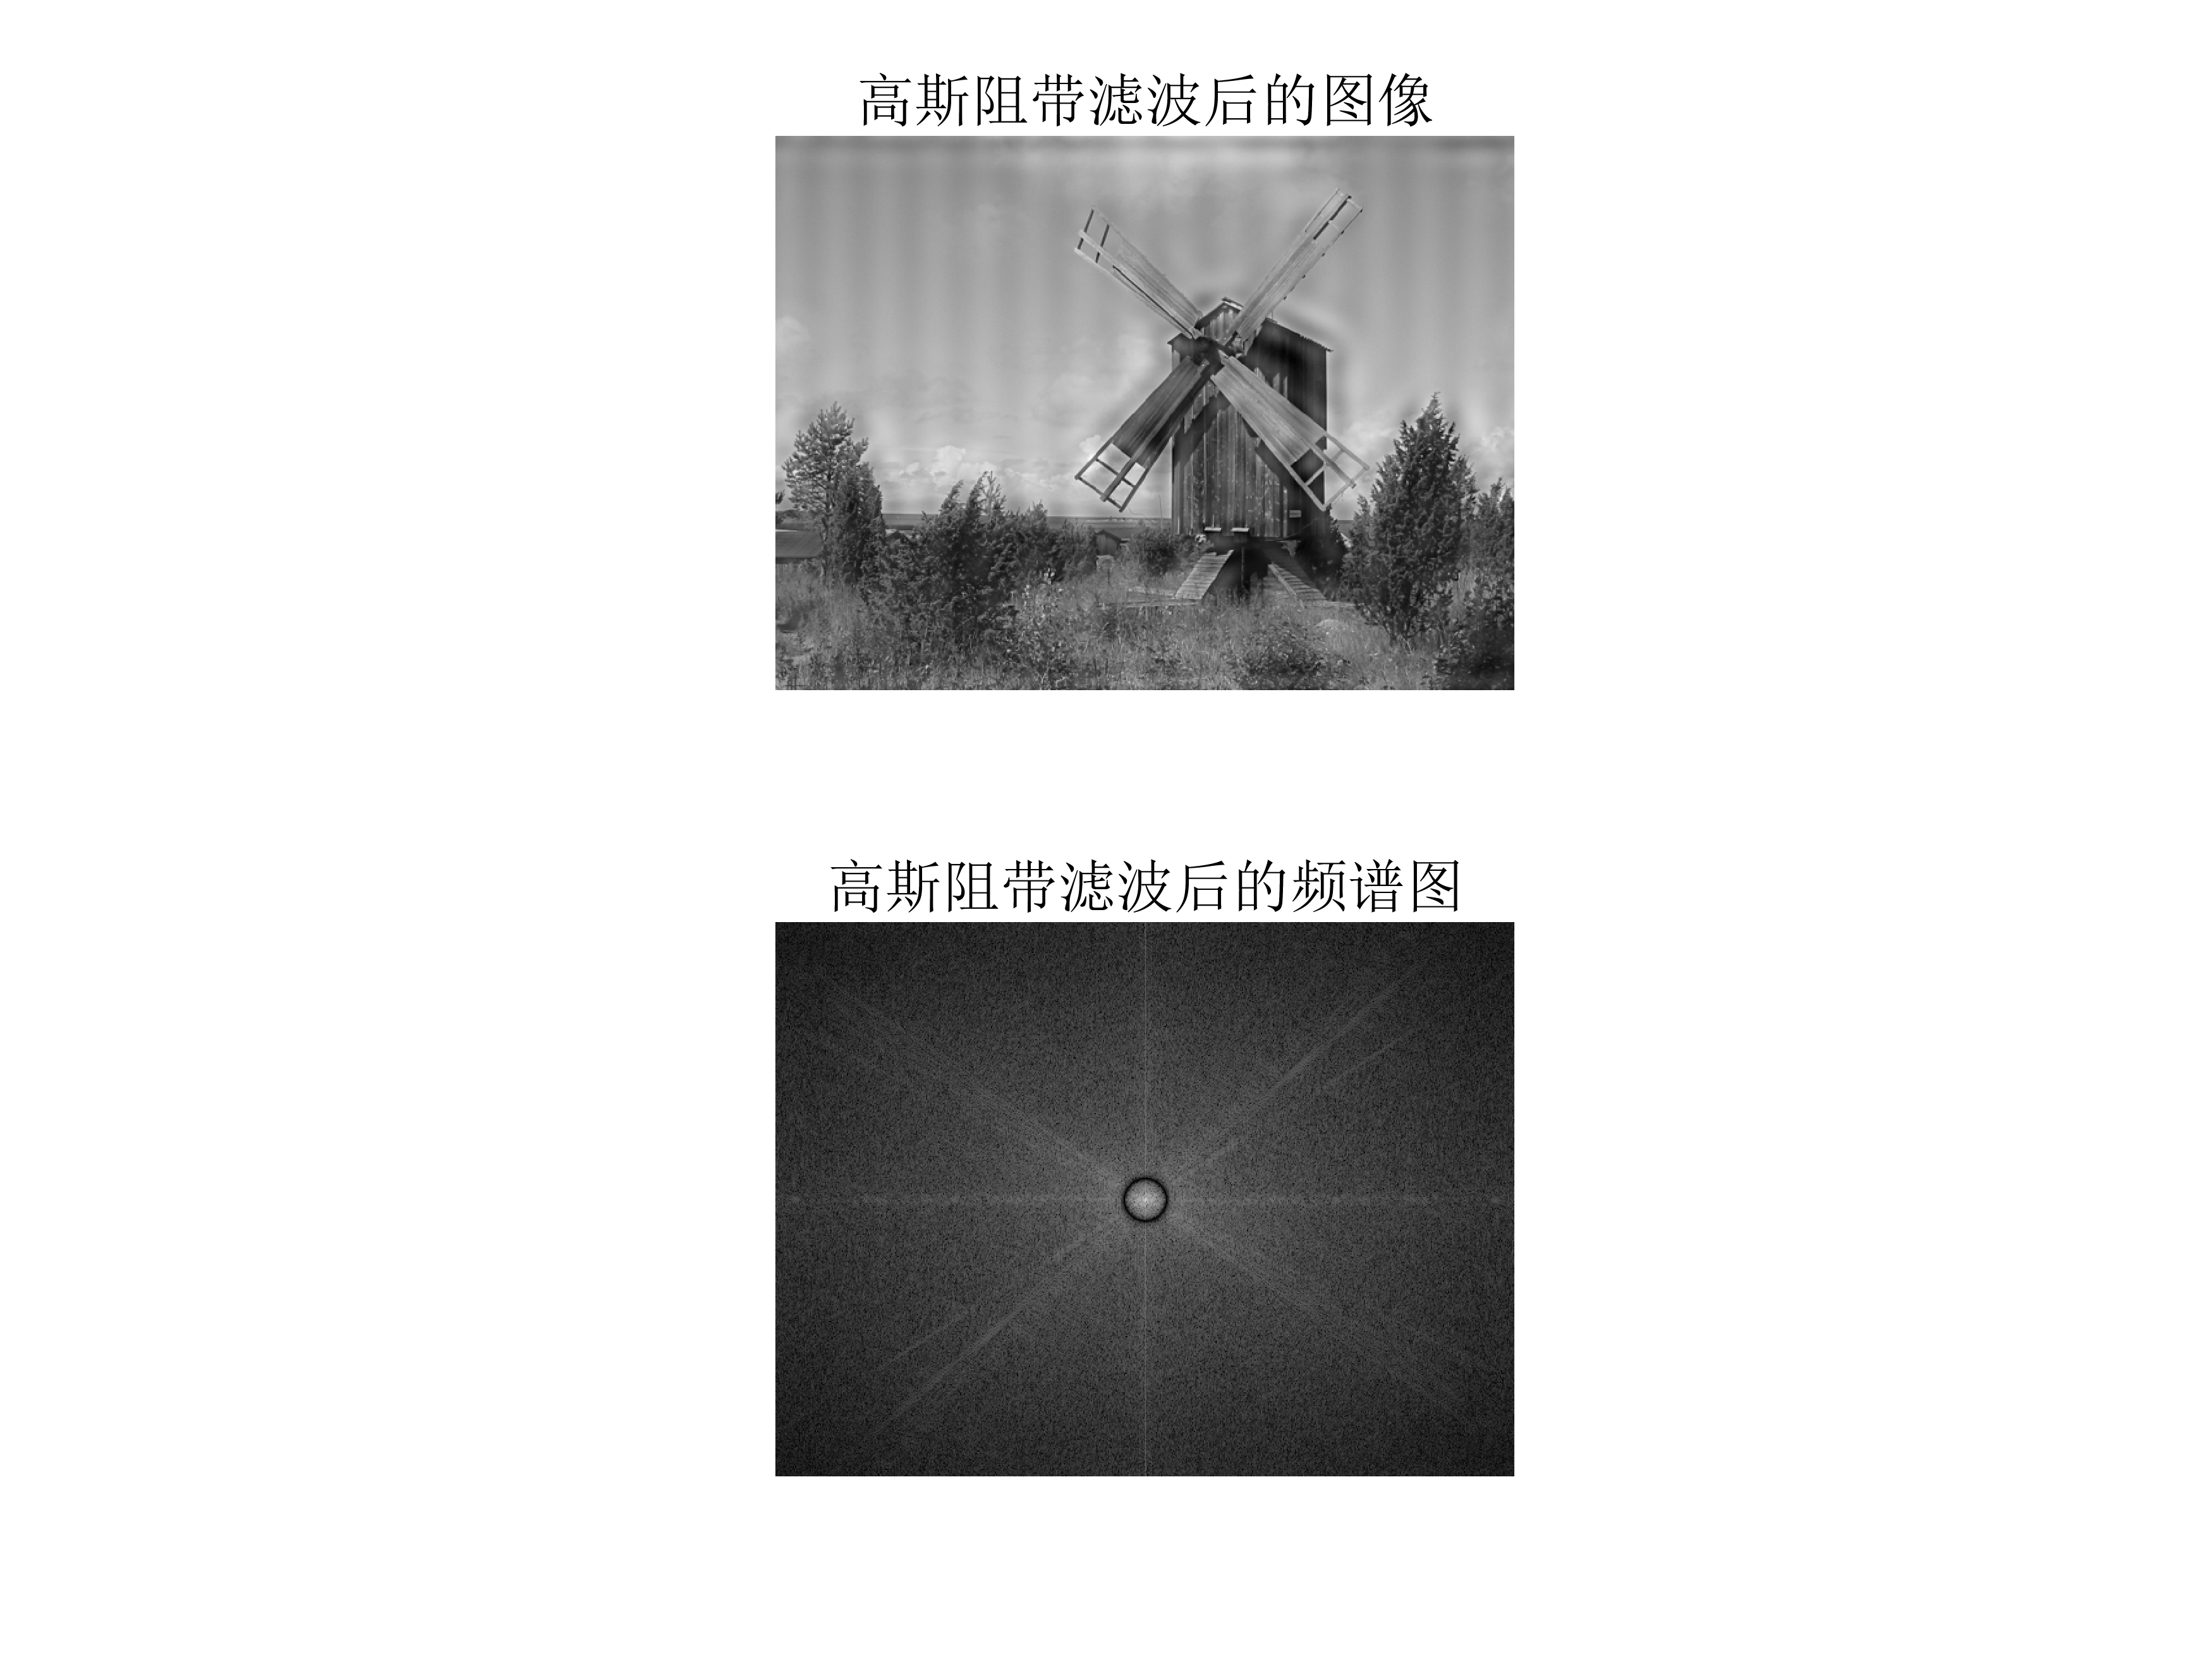
\includegraphics[scale=0.4]{./Gaussian_filtered_img.png}
%                                    %\caption{原图3}
%                                \end{minipage}
%                            }
%                            \subfigure[高斯带阻滤波后的频谱图]{
%                                \begin{minipage}{0.45\linewidth}
%                                    \centering
%                                    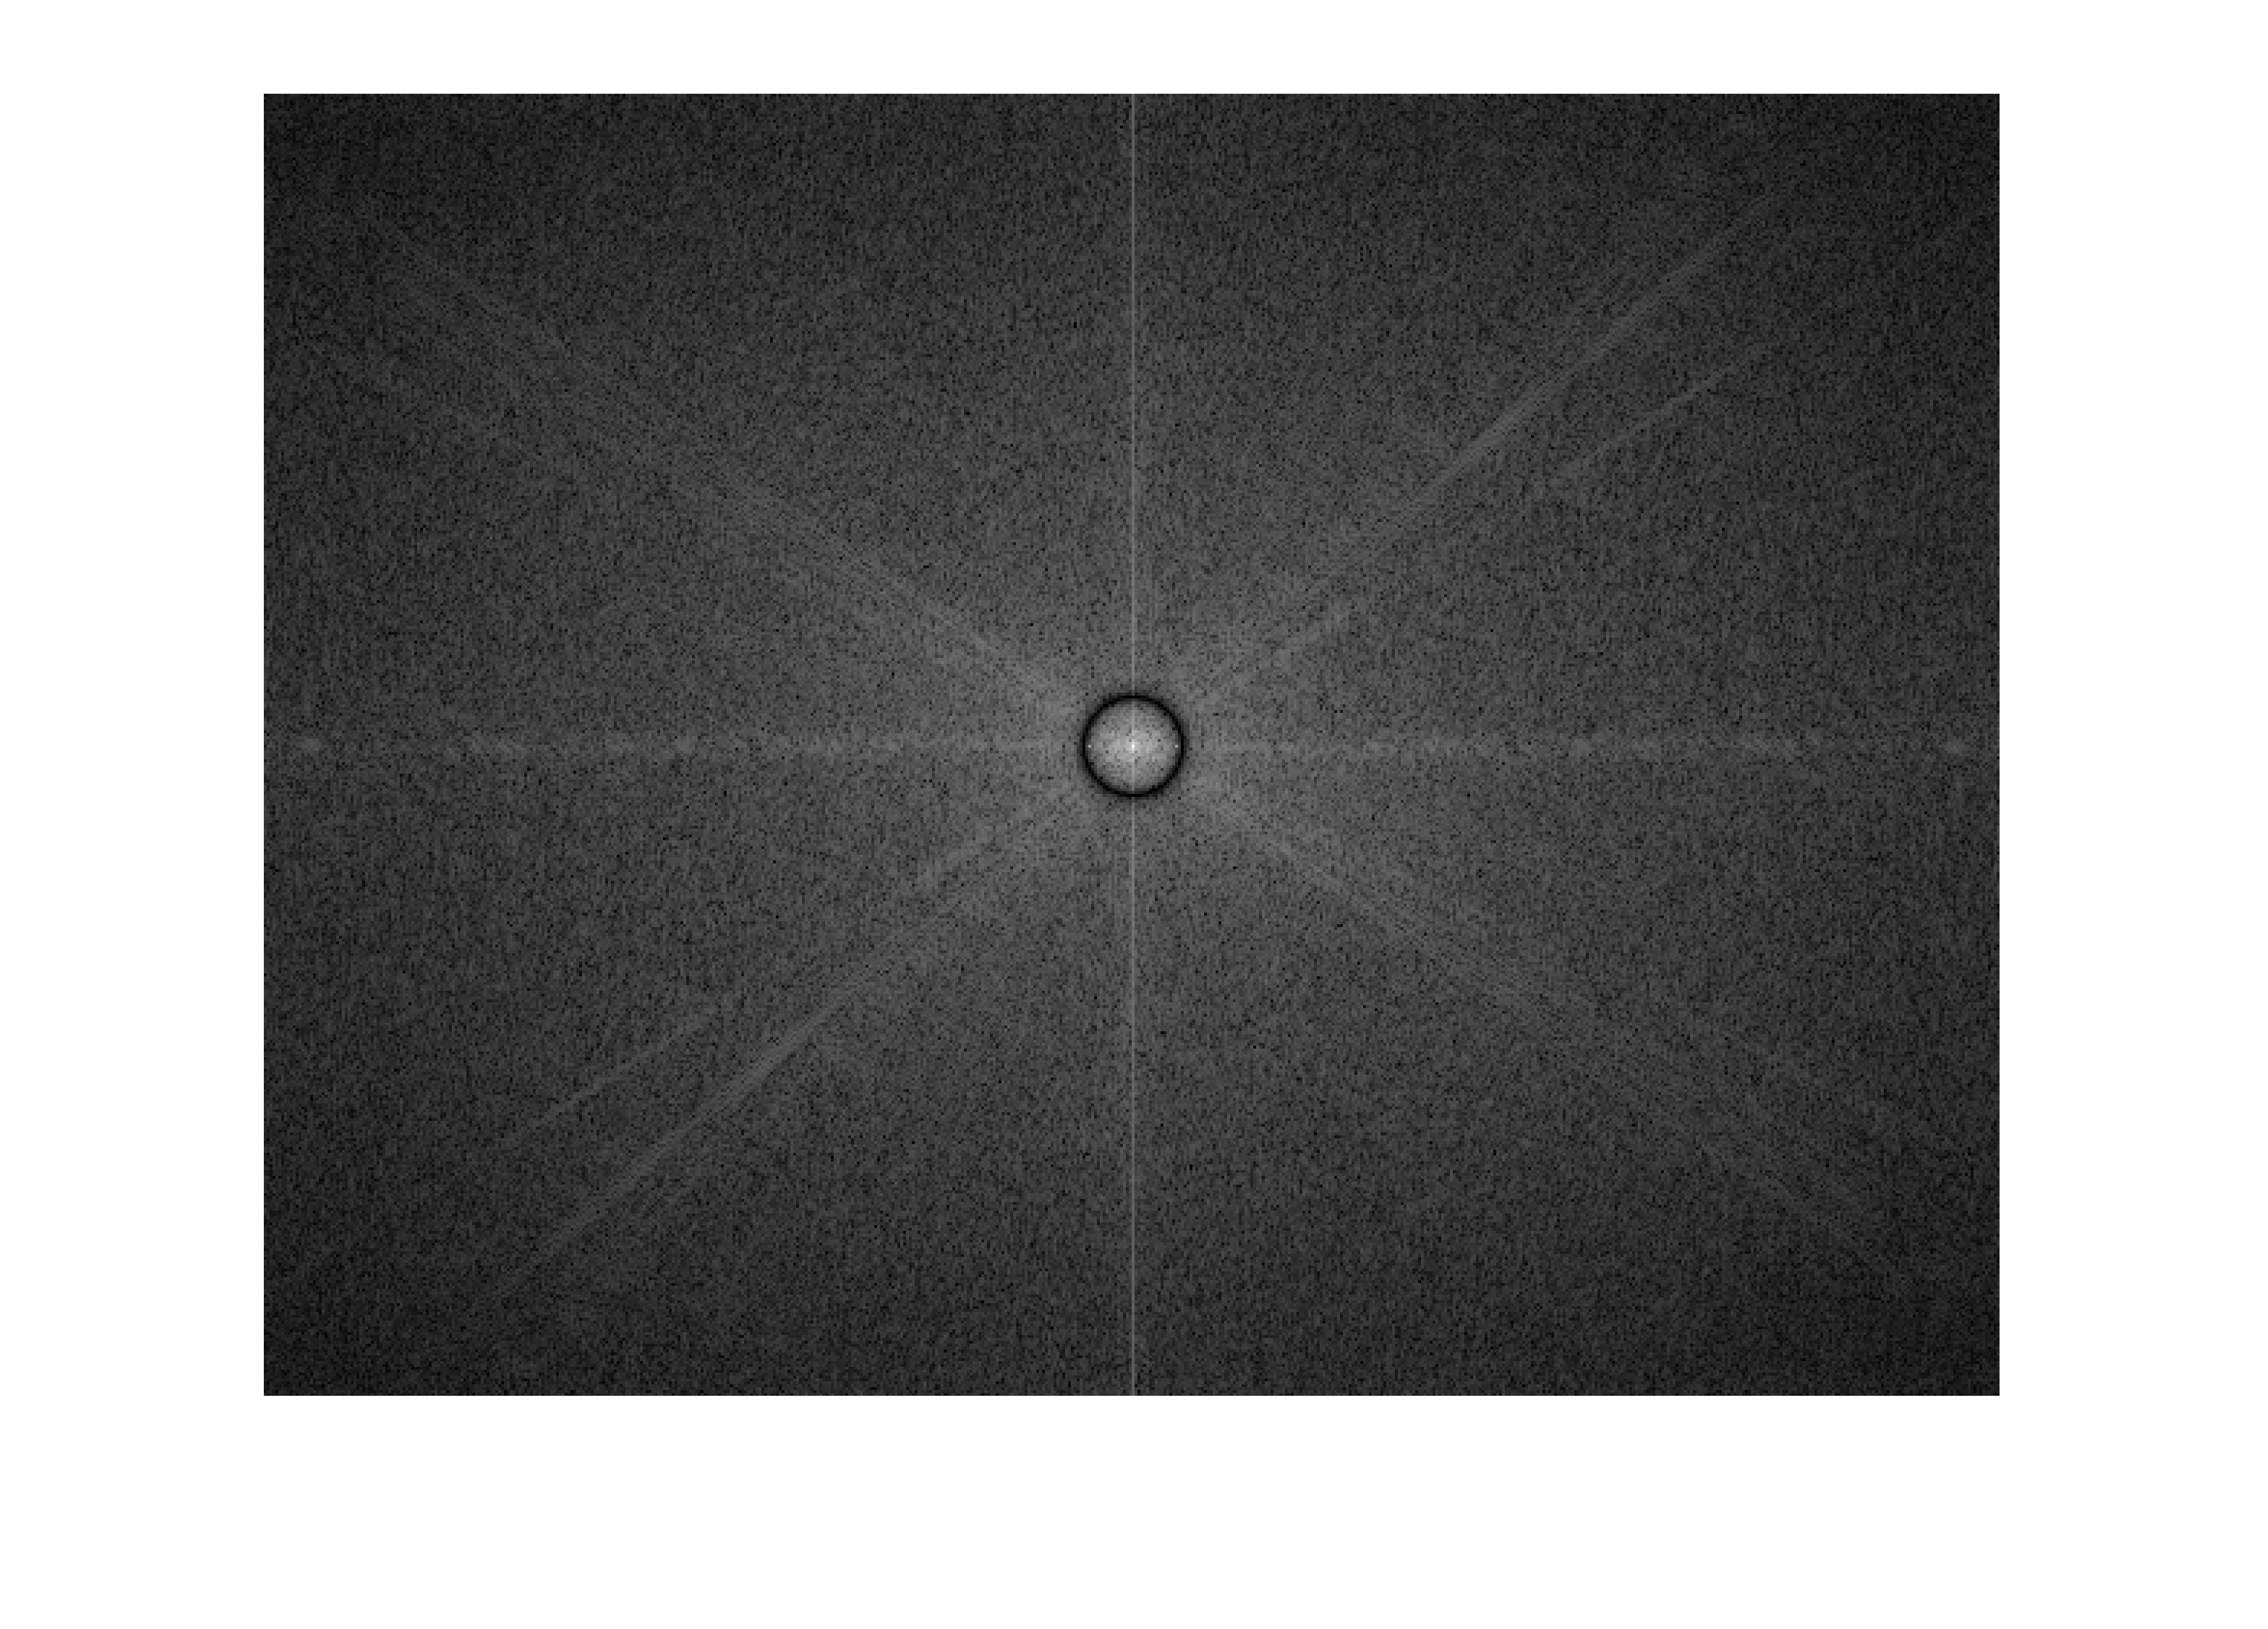
\includegraphics[scale=0.4]{./Gaussian_filtered_spectrum.png}
%                                    %\caption{结果3}
%                                    \label{res4-4}
%                                \end{minipage}
%                            }
%                            
%                            \caption{测试结果}
%                            \label{gaussian}
%                        \end{figure}                              
%                        
    
                            
                                   

	\section{总结}
		
        \indent 本次实验是用哈尔小波变换对图像边缘进行增强。从图\ref{n_eq_4}到图\ref{n_eq_10}可以看出,小波变换的阶数越高,消除近似分量所损失的信息和能量就越少,反变换得到的结果也就越完整。
        
        \indent 同时也可以从本次实验中看出,用小波变换对图像进行操作要比用傅里叶变换对图像进行操作更灵活。以本次的哈尔变换为例,我们不仅可以改变图像的频率分量,还能针对方向(水平、垂直、对角)对其做出改变。可见小波变换能够将位置信息引入到频率域,为频率域的图像处理方法拓展了空间。
        
%			\begin{figure}[H]
%				\centering 
%				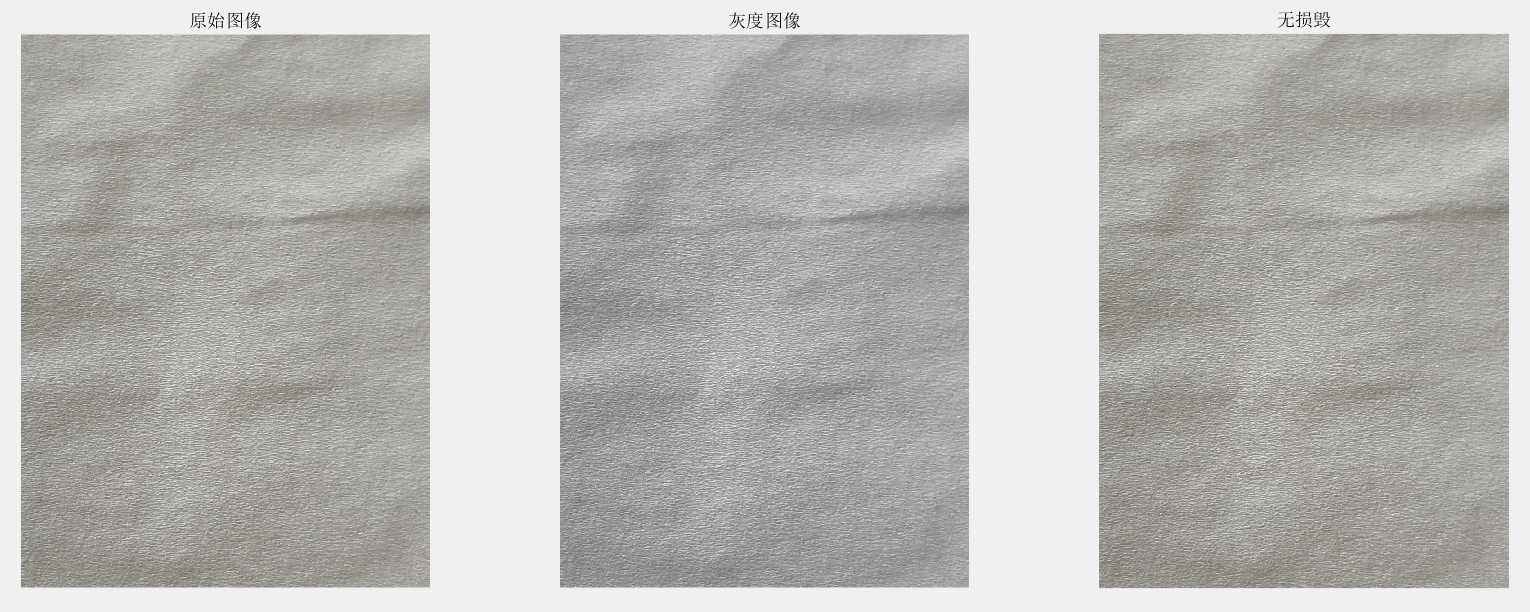
\includegraphics[scale=0.4]{res4.png} 
%				\caption{结果4} 
%				\label{res4}
%			\end{figure}
		

		
%			\begin{figure}[H]
%				\centering 
%				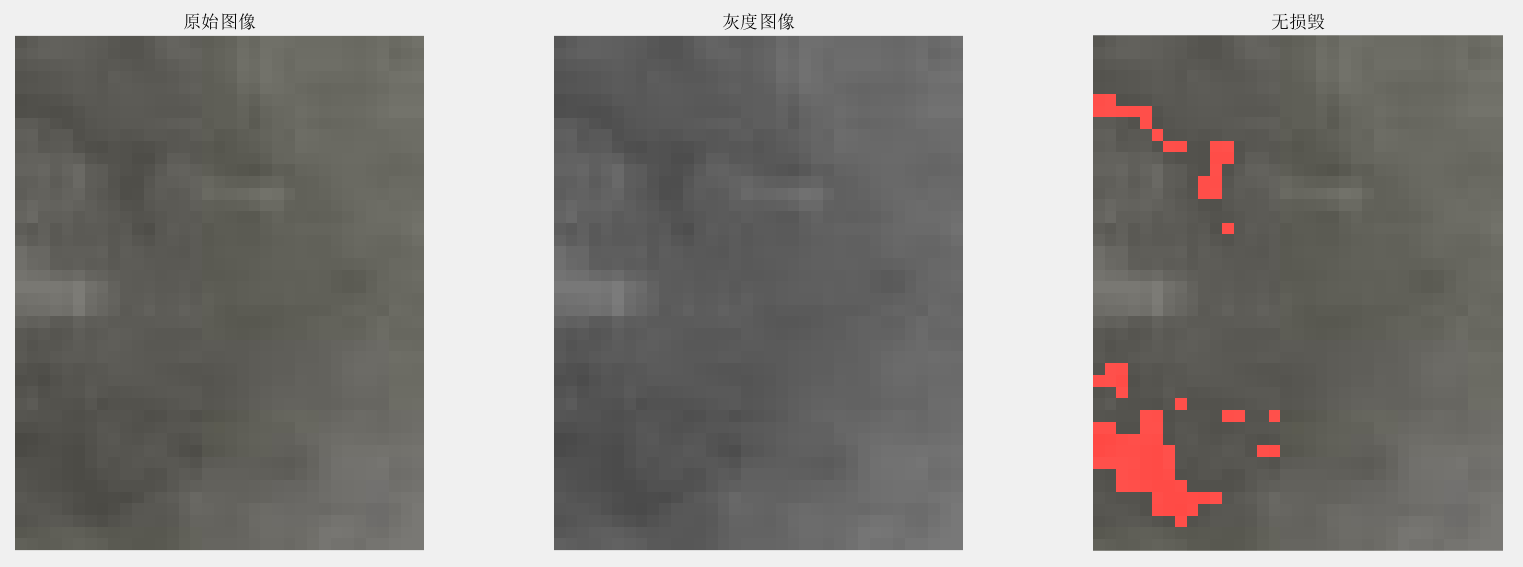
\includegraphics[scale=0.4]{res6.png} 
%				\caption{结果6(截取自结果5的阴影部分)} 
%				\label{res6}
%			\end{figure}
	
	
% 中文文献多个作者用中文逗号“,”连接
%\bibliography{ref.bib}
%\bibliographystyle{abbrv}
\bibliography{ref.bib}


\end{document}